\documentclass[twoside,11pt,a4paper]{article}
\usepackage[utf8]{inputenc}
\usepackage[english]{babel}
\usepackage{amsmath}
\usepackage{amsfonts}
\usepackage{amssymb}
\usepackage{graphicx}		% for \includegraphics
\usepackage{subcaption}		% for subfigures
\usepackage{listings}		% for \lstlisting
\usepackage{xcolor}			% for \color
\usepackage[hidelinks]{hyperref}		% for \url
\usepackage[a4paper, width=15cm, top=3cm, bottom=3cm]{geometry} %inner=3cm,outer=2cm
\usepackage[section]{placeins}
\usepackage{fancyhdr}
\usepackage{array}			% to fix column widths

%  === NEW COMMANDS ===

\newcommand{\todo}[1]{\textit{TODO: #1}}
\newcommand{\maybe}[1]{\textit{(maybe ? #1)}}
\newcommand{\refneeded}{\textit{`reference needed`}}

\newcommand{\java}[1]{\textsf{#1}}

\newcommand{\sql}[1]{\texttt{#1}}

\newcommand{\pls}[1]{\small\texttt{#1}\normalsize}
\newcommand{\plstype}[1]{\pls{#1}}
\newcommand{\varchar}{\plstype{VARCHAR2}}
\newcommand{\oranum}{\plstype{NUMBER}}
\newcommand{\plsi}{\plstype{PLS\_INTEGER}}
\newcommand{\simpleint}{\plstype{SIMPLE\_INTEGER}}
\newcommand{\plsnull}{\pls{NULL}}
\newcommand{\notnull}{\pls{NOT NULL}}

\newcommand{\jitted}{JITted}
\newcommand{\etal}{\textit{et al.}}

\newcommand{\benchsystem}[1]{\textsf{#1}}
\newcommand{\pvm}{\benchsystem{pvm}}
\newcommand{\pvmg}{\benchsystem{pvm-pragma}}
\newcommand{\ncomp}{\benchsystem{ncomp}}
\newcommand{\ncpg}{\benchsystem{ncomp-pragma}}
\newcommand{\truffle}{\benchsystem{truffle}}

\newcommand{\bench}[1]{\textsf{#1}}
\newcolumntype{R}{>{\raggedleft\arraybackslash}m{9mm}}
\newcolumntype{P}[1]{>{\raggedleft\arraybackslash}p{#1}}
%\let\newline\\\arraybackslash\hspace{0pt}

\newcommand{\maintitle}[1]{{\fontfamily{ppl}\selectfont\textbf{#1}}}
\newcommand{\startsection}[1]{
	\cleardoublepage
	\section{#1}
	\thispagestyle{basic}
}
\newcommand{\review}[1]{\textbf{\color{red} [#1]}}

\newcommand{\bibpaper}[4]{
	\bibitem{#1}	% reference
		#2.		% authors
		#3.		% publication name
		#4.		% date and other comments
}

\newcommand{\bibproceeding}[5]{
	\bibitem{#1}	% reference
		#2.		% authors
		#3.		% publication name
		In \textit{#4},		% conference
		#5.		% date and other comments
}

\newcommand{\bibbook}[5]{
	\bibitem{#1}	% reference
		#2.		% authors
		\textit{#3}.		% name
		#4,		% publisher
		#5.		% date and other comments
}

\newcommand{\biburl}[3] {
	\bibitem{#1}	% reference
		#2.\newline{}		% name
		\url{#3}		% url
}


\lstdefinestyle{PLSQL}{
	language=SQL,
	tabsize=4,
	keywordstyle=\color{brown},
	morekeywords={PROCEDURE,FUNCTION,IS,BEGIN,END,LOOP,FOR,WHILE},
	frame=L
}

\lstdefinestyle{SQL}{
	language=SQL,
	keywordstyle=\color{orange},
	basicstyle=\ttfamily
}

%\newfontfamily\javafont[Scale=0.7]{Courier}
%\newfontfamily\javafontinline[Scale=0.8]{Courier New}
\definecolor{java_comment}{rgb}{0.12, 0.38, 0.18}
\definecolor{java_keyword}{rgb}{0.37, 0.08, 0.98}
\definecolor{java_string}{rgb}{0.06, 0.10, 0.98}
\lstdefinestyle{Java}{
	language=Java,
	tabsize=4,
	numberstyle=\tiny,
	basicstyle=\sffamily\small,
	stringstyle=\color{java_string},
	keywordstyle=\color{java_keyword},
	commentstyle=\color{java_comment}\itshape
}

% === FORMATTING ===

\author{Hugo Kapp 227942}
\title{High-performance PL/SQL interpreter for Graal using Truffle}
\date{August 18, 2017}

\fancypagestyle{content}{ %
	\fancyhf{}
	\fancyhead[LE]{\leftmark}
	\fancyhead[RO]{\rightmark}
	\fancyfoot[LE,RO]{\thepage}
	\renewcommand{\headrulewidth}{1pt} % remove lines as well
	\renewcommand{\footrulewidth}{0pt}
}

\fancypagestyle{basic}{ %
	\fancyhf{} % remove everything
	\renewcommand{\headrulewidth}{0pt} % remove lines as well
	\renewcommand{\footrulewidth}{0pt}
	\fancyfoot[LE,RO]{\thepage}
}

\pagestyle{basic}

% === DOCUMENT BEGINS ===

\begin{document}

%\maketitle
\pagenumbering{roman}
\begin{titlepage}
    \begin{center}
		\begin{minipage}{1.1\textwidth}
  \centering
  \hspace{-1.3cm}
  $\vcenter{\hbox{
\includegraphics[width=7cm]{./pics/EPFL-Logo.jpg}}}$
  \hspace{2.5cm}
  $\vcenter{\hbox{
\includegraphics[width=6.5cm]{./pics/oracle-logo.png}}}$
\end{minipage}    
    
%        \begin{figure}
%        \centering
%        
\includegraphics[width=6cm]{./pics/EPFL-Logo.jpg}
%        \hfill
%        
\includegraphics[width=6cm]{./pics/oracle-logo.png}
%        \end{figure}
        
        \vspace*{3.5cm}
        
        \huge
        \maintitle{High-performance PL/SQL interpreter for Graal using Truffle}
        %{\fontfamily{ppl}\selectfont\textbf{High-performance PL/SQL interpreter for Graal using Truffle}}
        
        \vspace{2cm}
        
        \LARGE
        \maintitle{Hugo Kapp}
        
        \vspace{2.5cm}
        
        \Large
        Master Thesis\\
        \vspace{0.2cm}
        Department of Computer Science\\
        \vspace{0.2cm}
        EPFL
        
		\vfill       
		\normalsize
        Work done during an internship at\\
        \vspace{0.2cm}
        \Large Oracle Labs \large
        
        \vspace{0.3cm}
        
        %A thesis presented for the degree of\\
        %Doctor of Philosophy
        
        %\vspace{0.8cm}
        
        %\includegraphics[width=0.4\textwidth]{university}
        
		\begin{itemize}
		\centering
		\item[Professor] Martin Odersky
		\item[EPFL Supervisor] Denys Shabalin
		\item[Industry Supervisor] Laurent Daynès
		\end{itemize}
        
	    \vspace{0.3cm}
    
		Spring 2017
		
	    \end{center}
	
\end{titlepage}

\cleardoublepage

\vspace*{1cm}
\section*{\hfil Abstract\hfil}
\label{sec:abstract}
%\addcontentsline{toc}{section}{Abstract}

\vspace{0.5cm}

In the age of Internet and ever-growing storage facilities, performance of database operations are critical. Much work has been done in the past decades to improve significantly the execution speed of data queries. To this end, specialized query languages have been designed, which allow for very specific, fine-tuned optimizations. However, such languages tend to be limited in expressiveness, and make the writing of simple data validation or processing tasks very difficult. Procedural extensions to such querying languages lift this constraint, but their additional generality makes them a more complex target for optimizations.

We present in this thesis a more efficient way to execute procedural programs inside the database, using modern \textit{just-in-time} (JIT) compilation, code specialization and aggressive speculative optimizations. Our work is based on the Truffle language framework and the Graal VM, two cutting edge techonologies developped at Oracle Labs. We implement a subset of the PL/SQL language, the procedural extension to SQL in Oracle databases using these tools. We show that the combination of dynamic optimization and code specialization can improve performance over the best PL/SQL execution engines available today. Furthermore, we assess the possibilities and benefits of type specialization inside a statically-typed language, that has a very complex type system. We also demonstrate that it is possible inside runtime-specialized systems to change between different data representations for the same data type at runtime, and that this can be used to improve performance significantly. Finally, we show that, using the Truffle framework and the capabilities of the Graal compiler, it is possible to write such execution engines with a small amount of high-level Java code.

%current, generic native compiled option.

\newpage
\section*{Acknowledgements}
\label{sec:acknowledgements}
%\addcontentsline{toc}{section}{\nameref{sec:acknowledgements}}
%\markboth{Acknowledgements}{Acknowledgements}

I would like to thank Professor Martin Odersky for allowing me to do my Masters thesis in his prestigious lab.

I would then like to thank Denys Shabalin for his supervision during this project, and helping me keep track of time and due dates during my internship.

I am most grateful to Laurent Daynès for helping me throughout this project. His vast knowledge on both databases and compilers were very helpful to aid my understanding of the systems at hand. I wish him all the best for the continuation of his project.

Finally, I want to show all my gratitude to my parents, who helped me get through my studies and every stage of my life.

\newpage

\tableofcontents

\newpage

\listoffigures

%\newpage

%\listoftables

%\cleardoublepage
\startsection{Introduction}
\pagenumbering{arabic}
\pagestyle{content}
%\thispagestyle{basic}

%\textbf{Problematic / problem of the project :}
%\begin{itemize}
%\item Can we use different specialized data representations for the same data type to achieve high-performance ?
%\item Can this be applied specifically to data-driven programming like PL/SQL ?
%\item Can it be done with comparable (or even better) memory consumption ?
%\end{itemize}
%
%Answer should be yes, with Truffle and Graal this is even made kind of easy.
%Last point must still be validated.

Databases today are a central part of any application. They are used to store information about customers, transactions, identifiers and passwords, and much more. With large and cheap memory storage, and a widespread access to the Internet, these tables typically hold millions of records. It is therefore crucial that getting access to this data and performing simple processing steps is as efficient as possible.% Simple processing tasks, like validation and conversions of input values, or expansion of missing records should also be done inside the database.

Query languages, like SQL, provide a very efficient way of fetching and modifying data. However, their limited expressiveness restricts the set of processing tasks that can be performed efficiently. To lift this restriction, procedural languages also running inside the database are usually added to allow for more flexibility, and to reduce the amount of communication between the database and its clients. Until recently, performance of these languages were not the main bottleneck. Now that databases start to fit in main-memory, their performance is becoming critical. However, the fact that they are full-fledged programming languages, with much more generality than querying languages, makes optimization much harder. Furthermore, frequent communications between the two kinds of languages incurs, on top of context switching overhead, a mismatch in data representation : space-optimized values provided by the database are typically not efficient when it comes to performing generic-purpse computation.
%and the need for computation efficient representations by the procedural languages makes the task of improving performance even harder.

In this project, we look at the Oracle database and its embedded procedural language called PL/SQL, and try to improve its performance. We do so by using the latest \textit{Just-In-Time} compilation technology, code specialization, and runtime data representation specialization. This is done by implementing an efficient AST interpreter using the Truffle language framework, a rich API to write self-specializing interpreters. PL/SQL programs are then run on top of the Graal VM, which uses a new JIT compiler for Java bytecode that aims at bringing more languages to the JVM. It uses aggressive speculative optimizations to execute programs at high speed, and enables foreign languages implemented using the Truffle framework to benefit directly from these optimizations. Truffle and Graal are two open-source projects, actively developped at Oracle Labs. We tackle the specific problem of having data representations not suited for computation by performing runtime data representation specialization. This allows us to use multiple value representations for the same data type, and choose the best fit for the current program at runtime.
%We use the speculative optimizations provided by the Graal compiler, as well as code specialization framework of Truffle, two projects developped at Oracle Labs, to implement an efficient PL/SQL interpreter. 

This thesis will answer the following questions :
\begin{itemize}
\item Can a language interpreter, based on runtime code specialization, improve execution time of the said language ? And by how much ?
\item Is this true, even in the very specific context of data-centric languages like PL/SQL?
\item Can we use different specialized data representations for the same type, and change them at runtime ? What kind of impact does this have on the execution of the program ?
\end{itemize}

%These querying languages typically have very high performance, but low expressiveness. To allow for 
%
%%This has become an even more pressing issue as \textit{big data} and machine learning gain in popularity, performing statistics and analysis on huge amounts of data.
%
%Typical queries in databases are very efficient, through the use of specific languages, like SQL. However, they have a limited expressiveness, which makes computation infeasible. To increase the programmability of languages running inside the database, i.e. as close to the data as possible, database users tend to use a procedural language like PL/SQL. Although this removes the cost of transfering data outside the database for processing, the implementation of such languages must be guaranteed to be very efficient. Many specific optimizations are performed, tailored to classic database uses, but this is not enough.
%
%
%
%The typical way to access this data is through a querying language, the most popular being SQL. Queries made using such a language are very efficient, but this is achieved by allowing (relatively) simple queries only, with a very restrained syntax. No variables can be used, and no code can be reused, which makes the writing of complex queries very hard. To solve this problem, 
%
%PL/SQL is an imperative language that runs inside Oracle databases. Its goal is to query, manipulate and process data efficiently. Of course, because it can manage millions of records, execution speed of such programs is a top priority, and providing a high-performance implementation of such a language a necessity.
%
%Although many optimizations have been added inside Oracle's execution engine to improve the performance of PL/SQL programs, much room for improvement still remains. An interpreter-based solution gives very poor performance, while a native compiled option still makes heavy calls into a compex shared library. The specificity of the type system, which must accomodate for space-optimized values coming from database tables, does not make this task easy.
%
%In this project, we describe and implement a solution based on \textit{Just-In-Time} (JIT) compilation and speculative optimizations. We tackle the representation issue by using runtime data representation specialization, and use runtime code specialization to dramatically improve the execution speed. The system is based on the Truffle framework and Graal VM, two projects developped at Oracle Labs.

\vspace{1cm}

We complete this introduction by listing the precise goals of this project and discussing previous work. We then set the background for this project. First, we give a quick overview of the PL/SQL language and its specificities in Section 2. Then, we describe the relevant aspects of the Truffle and Graal ecosystem in Section 3. After that, we give details on our approach for a first interpreter using only integer types in Section 4, and complete that basic system with the \varchar{} type in Section 5. We then assess the performance of this solution in Section 6. Finally, we give directions for continuation of this project in Section 7, before concluding in Section 8.

\subsection{Goals}

%\begin{itemize}
%\item propose incremental replacement to classic PL/SQL interpreter, with improved performance
%\item show specialized representation for the same data type can improve performance
%%\item maybe ? (depends on benchmarking results for that) show that on-the-fly code replacement and optimization gives better performance than what is reachable with AOT compiler, especially for very specific patterns
%\item Analyze ease of writing and memory consumption of such a solution, in the context of the Graal/Truffle environment
%\item Only interested in the UDF case, basic calls not very interesting (not our target in this project, which focuses on data-driven programming)
%\item (data) specialization useful in small programs ?
%\item produce a prototype that allows UDF calls ?
%\end{itemize}

We have multiple goals for this project. The first is to improve the performance of PL/SQL programs beyond what is currently reachable with the options available in the Oracle database.

The Oracle database already provides high-performance execution modes for PL/SQL programs, namely a native compilation option that compiles the PL/SQL programs down to machine code. It also supports many programmer hints and options, which improve the execution time significantly. We show that current JIT technology, using advanced runtime optimizations, can go faster than the solutions compiled ahead-of-time. We demonstrate how runtime code and data specialization can help improve performance by focusing only on the relevant parts of the code. We confirm that, even in very small and data-intensive programs like the ones typically run with PL/SQL, runtime data representation specialization can improve performance substantially.

We limit ourselves to specific programs, which represent the typical uses of PL/SQL inside the database. Contrary to general-purpose languages, that are used to write computation intensive and generally long programs, PL/SQL functions are usually called inside SQL queries. We will focus on small functions, called as UDFs (User-Defined Functions), to demonstrate the advantage of our solution on a typical workload.

%Implementing the interpreter with the Truffle framework also allows for simple integration with other languages. This opens the opportunity for PL/SQL legacy programs to get direct and cheap access to newly written programs, in any language of the programmer's choosing. Because Graal and Truffle are built to be multi-languages platforms, this is 

However, we do not provide a full re-implementation of the language. Instead, the system designed here should be an incremental replacement of the classic PL/SQL execution engines. We implement a subset of the language only, which should be representative enough, as well as easily extensible. For example, we do not provide support for any SQL queries inside the PL/SQL code, and focus on procedural programs only. This incremental subset approach allows for a smoother integration of our system into the Oracle database, while keeping the original engines as backup.

Finally, this project also serves as an exploration of the Graal and Truffle framework. We show that implementing a high-performance AST interpreter is possible, and made simple by writing everything in a high-level programming language like Java, using the Truffle API. We demonstrate that complex specialization optimization are easy to write, and can be tailored to our needs to improve performance further. We also investigate the benefits of code specialization in a statically-typed context, a technique usually reserved for dynamically-typed languages.

\subsection{Previous work}

%Laurent's plan:
%\begin{itemize}
%\item runtime specialization in programming language with JIT
%\item runtime specialization of type representation in general (in plsql, in db)
%\end{itemize}
%
%Different than dbjs in :
%\begin{itemize}
%\item statically typed language (Truffle not really built for that)
%\item PL/SQL already running in the DB (improvement instead of new func : possible to compare to existing C implementation)
%\item \textbf{Language specific to data processing} (JS itself is general-purpose)
%\item everything is implemented by us (JS interpreter implemented by GraalJS team, so no optimizations made directly for database integration / data-centric workload)
%\item null-support (also empty-null-stirng semantics)
%\end{itemize}
%
%\begin{itemize}
%\item other truffle implementation of languages
%\item walnut of course (dbjs)
%\end{itemize}

Although many optimizations have been added to the PL/SQL compiler and execution engine over the years, very few are documented. This is due to the technology being a proprietary product, owned by Oracle. The best publication for such matter is the white paper by Charles Whetherell \cite{freedomplsopt}. The author defines the relaxed assumptions on correctness that were made to allow more room for optimization in the PL/SQL compiler. We would reuse his definition of \textit{freedom} if we were to argue about the correctness of our own interpreter.

Other variants of procedural extension of SQL in other databases share the same kind of compilation and execution options. Transact-SQL \cite{tsqldoc}, which is Microsoft's extension to SQL, provides both an interpreted and a natively compiled mode. Like Oracle databases, the latter improves performance radically, and optimizations are performed for both execution alternatives. PostgreSQL only provides an AST interpreter for its procedural extension, called PL/pgSQL \cite{plpgsqldoc}. However, they started integrating just-in-time compilation into the database for executing SQL queries. Melnik \cite{postgresllvmjit} presented his results using a JIT compiler for LLVM to speed up query execution. Our approach goes in a similar direction, but we execute procedural programs, and do it from a higher-level representation.

%For these languages and PL/SQL, most of the focus for optimization is on interaction with SQL itself. Tight integration between the two is reinforced, in order to have inexpensive context switching.

Much work has been done in implenting runtime-specialized compilers and interpreters for various languages. The first example is the SELF \cite{self} compiler in 1992. The concept has been reused to improve the performance of modern, dynamically-typed languages, using JIT-technology. One such project is the IonMonkey \cite{jsvalue} JIT compiler for JavaScript, developped at Mozilla, which makes assumptions about argument values of function calls. Most of these projects focus on type specialization, as that is where there is the most room for optimization in dynamically-typed languages. \textit{Type specialization} performs optimizations based on the assumption that the type of an expression is always the same at execution time. Wang \etal{} \cite{rspec} use this technique to reduce the allocation overhead of the R interpreter, by performing boxing elimination with the runtime type information. Many JIT compilers have been implemented for dynamically typed languages to reap the most benefits from type specialization. We can cite Psyco \cite{psyco} for Python, Majic \cite{majic} for MatLab, and the work of Gal \etal{} on JavaScript \cite{gal, gal2}. Our work uses the Truffle framework and runs on the GraalVM, and many of the aforementioned languages have already been implemented using the same combination : Graal.JS \cite{trufflespec} for JavaScript, ZipPy \cite{zippy} for Python, FastR \cite{fastr} for R ...

This work has been done in the context of the Walnut project \cite{walnuthome}. Its goal is to integrate new programming languages into the Oracle database with high execution speed, using the Graal VM and Truffle framework. Their main focus to this day is on the JavaScript language, adding database bindings and interactions on top of the Graal.JS implementation. This is very close to what we present here with PL/SQL. However, there are major differences. First of all, they target a dynamically-typed language, which is not our case. We therefore show that the concept of specialization also has many benefits in a statically-typed context. Furthermore, we can account for the very speficic uses of PL/SQL and its tight integration with SQL and the database, for example in the representations used for various data types. We can then use this information to devise specific optimizations, which is not possible in a generic-purpose language like JavaScript. Finally, our prototype is a proposed replacement for something that already exists in the database. Therefore, it is, and must be, and improvement over the existing system. This is a very different approach than trying to integrate something new into the database, with no reference and no backup to hold on to.


%\cleardoublepage
\startsection{The PL/SQL language}

We give in this section an overview of the PL/SQL language, and explain its most relevant features for this project.

\subsection{History}

Today, databases are everywhere. They support the data we fetch from the internet, stores large amounts of data for companies, and keeps track of user and customer informations. But the concept of databases is not a recent one. The term appeared in the 1960's, first as "data-base", and eventually became a single word. But the databases changed a lot since then, and the ones we are accustomed to are very different than the ones used in the past.

The vast majority of databases in use today are what is called \textit{relational databases}, which were invented by Codd in 1970 \cite{codd70}. This new way of storing data uses multiple different tables which consists of a number of columns. Each column define the kind of elements it stores. Tables and columns are usually referred to by names, and are created using a specific language, called DML (Data Manipulation Language). This language is specific to the database system used. This basic system has been extended over the years, but its foundations remain.

\begin{figure}[hb]
	\centering
	
	\begin{subfigure}[h]{\textwidth}
		\centering
		\begin{lstlisting}[style=SQL]
CREATE TABLE emp (name VARCHAR2, salary NUMBER);
		\end{lstlisting}
	\end{subfigure}
	
%	\vspace{0.4cm}
	
	\begin{subfigure}[h]{\textwidth}
		\centering
		\begin{tabular}{| l | r |}
			\hline
			name & salary \\
			\hline
			'John Johnson' & 2000 \\
			'Ali Baba' & 4000 \\
			'John Doe' & \plsnull{} \\
			'Sarah Connor' & 8000 \\
			\hline
		\end{tabular}
	\end{subfigure}

	\caption{Example of a database table, and its corresponding DML statement}
	
\end{figure}

Information can then be retrieved from such tables using a \textit{querying language}. The most popular and widespread querying language today is SQL, which stands for Structured Query Language. Its most basic feature is the \sql{SELECT} statement, which allows to fetch data from a specific table under some user-defined constraints. This was the tool of choice of database users and managers to get the information stored in their database, and it still is today.

However, as is the case for every querying language, SQL has many limitations. Even though it allows for a wide variety of constraints, that can then be set on multiple tables at once, and lets the query issuer decide on which columns' data to fetch and which to ignore, and even apply basic operators on these result, some more complex queries can just not be done. On another level, code reuse is impossible, as queries are stand-alone programs, and are self-contained. Because SQL is not a programming language, it does not have variables or any kind of control-flow operators. Finally, SQL is very specific and distant from traditional programming language. Database users then need to learn SQL and its specificities before being able to use it fully.

\subsection{A database embedded language}

As described above, the need for a programming language that could manipulate the data stored and generate queries was strong. When faced with this problem, programmers did a very simple thing : they used their preferred programming language (e.g. C or Java), established a connection with the distant database as the client would have done manually, and start issuing queries as strings over the network. This solution, though very clean because of the separation between the various systems, and the reuse of existing languages and compilers, led to poor performance and network saturation.

%Although many features have been added over the years to increase the expressiveness of SQL, making a lot of task simple to write in SQL only, some of these tasks had to be completed before such support was added, or is still easier to write in a classic programming language form. Indeed, training programmers to write complex queries is both long and error-prone. Writing these tasks in a language that they are more familiar with would be simpler.

%The reason this solution is not feasible when performance is important is due to the data transfer model of relational databases and SQL. Because the database is distant, connection between the client application and the database must be remote (e.g. on the internet through IP packets). After that connection is established, the client application, written in some general-purpose language, starts issuing a query. This query is received in the database, compiled, and performed on the stored data. But all found data is not directly sent over the network : it is sent in batches when the processing application needs it. The client application will then receive some of the data, which might trigger another query ... The round-trip time between the client and the database is ruining the performance of the computation.

To fix this issue, the idea was to add, inside the database, a language that would be specialized for handling data and issuing queries. Because this language runs inside the database, nothing needs to be sent over the network. Everything remains local to one  machine (or a cluster of machines), which dramatically increases performance. In Oracle databases, this language is PL/SQL, where "PL" stands for Procedural Language.

PL/SQL is a statically-typed imperative language, with a support for SQL queries and data, table and tuple manipulation. It is based on the Ada programming language \cite{adadoc}, and has very similar syntax. It is compiled ahead-of-time into a bytecode language that is then interpreted by a virtual machine, called the PVM (for PL/SQL Virtual Machine). It has all the common features of an imperative language, like conditional branches, loops, variables, function and procedure calls. It is also possible to define packages in PL/SQL. Many more features and constructs have been added in the following versions, like records and even objects. For a complete description of the language, its syntax and semantics, please refer to the Oracle PL/SQL documentation \cite{plsdoc}.

The tight coupling between the database and the language, and the fact that PL/SQL is tailored for data management and retrieval makes it a good target for very specific optimizations, and many have been added to the compiler over the years \cite{freedomplsopt}.

%Some of the types used in PL/SQL are direct SQL data types, which removes the overhead of converting them to a naturally understood representation (the stored representation of values in columns is optimized for space consumption, and is not made for direct computation on these). 

%Because PL/SQL is a long-lived language, it has evolved over the years. Support for more high-level constructs has been added, like records, arrays and even objects.

\begin{figure}[t]
	\begin{lstlisting}[style=PLSQL]
PROCEDURE raise_all(fixed NUMBER, ratio NUMBER) IS
	raise NUMBER;
BEGIN
	FOR employee IN (SELECT name, salary FROM emp)
	LOOP
		raise := employee.salary * ratio + fixed;
		UPDATE emp
			SET salary = employee.salary + raise
			WHERE name = employee.name;
		send_raise_letter(raise, employee.name);
	END LOOP;
END;
	\end{lstlisting}
	
	\caption{Example of a PL/SQL program issuing SQL queries}
	\label{fig:plsraiseall}
\end{figure}

%\todo{talk about the drawbacks and problems of PL/SQL ?}

\subsection{Specificities \& differences with general-purpose languages}

As a programming language tightly integrated with the database, PL/SQL has many specificities compared to general-purpose programming languages.

First up, the programs and use cases are typically data-centric. This means that the ratio between code and data is inverted : very small programs may deal with millions of database entries, whereas classical programming languages have huge codebases but handle small amounts of data. In this sense, making optimizations is much more specific, as each program run will be very short, but still has to be very fast. The question then is "how much room for optimization do we have, if the ran programs are only a couple of lines long ?".

Even in this data-centric use of PL/SQL, there exists two main use-cases for the language. The first acts as a scripting language for SQL, with simple constructs. These programs vary widely in length, but typically have very few computation code in them, and mostly issue SQL queries. The program shown in Figure \ref{fig:plsraiseall} is an example of such use case. In this scenario, the performance of the PL/SQL execution is not that important. Most of the time will be spent executing the SQL queries, or switching context between SQL and PL/SQL.

In the second use case, PL/SQL functions act as UDFs (User-Defined Functions). We will call UDF calls to a (usually simple) PL/SQL function inside an SQL query. The benefit here is the ability to write the processing or condition of the SQL query in a simpler way, using typical programming language syntax. This also allows developers to reuse code in different queries. In this case, the SQL and PL/SQL engines must both be fast, and switching context between the two should be as lightweight as possible because the function call will be performed for every entry of the table. This is the case we will consider in this project. An example of this use case is given in Figure \ref{fig:plsudfexample}.

\begin{figure}[tb]
	\begin{subfigure}[h]{\textwidth}
		\begin{lstlisting}[style=PLSQL, frame=L]
FUNCTION pretty_print(salary NUMBER) RETURN VARCHAR2 IS
BEGIN
	CASE
		WHEN salary >= 1000000
			THEN RETURN TO_CHAR(salary / 1000000) || 'M';
		WHEN salary >= 1000
			THEN RETURN TO_CHAR(salary / 1000) || 'K';
		ELSE RETURN TO_CHAR(salary) || '$';
	END CASE;
END;
		\end{lstlisting}
	\end{subfigure}
	
	\begin{subfigure}[h]{\textwidth}
		\begin{lstlisting}[style=SQL]
SELECT pretty_print(salary) FROM emp;
		\end{lstlisting}
	\end{subfigure}
	
	\caption[Example of a procedural PL/SQL program, and how it can be used in a query as a UDF]{Example of a procedural PL/SQL program, and how it can be used in a query as a UDF. The '\sql{||}' is the concatenation operator.}
	\label{fig:plsudfexample}
\end{figure}

Another major difference is the fact that everything is done in the database, from the compilation to the execution. The user only sends the source code to the database, and waits for it to be compiled and stored there. Because everything is done and stored inside the database, it must follow the same rules as normal database elements. This means that the compiled code stored inside the system could be modified or removed concurrently to its use. This could be triggered by the function being modified, replaced, or totally removed, and can be done by any user who has the appropriate rights. These concurrency issues are taken care of by the database system, which performs the checks and take the appropriate action. But it means that a lot of runtime checks must be added, on top of the same kind of checks for data dependency. This makes the system much more complex and impacts performance.

%Runs that could hang or crash can also be difficult to debug. Now, many research and improvement has been made on reporting errors to the issuer of the query, but debugging what happens in the database remains a difficult process. 

%Finally, the workflow incurred by repeted database interaction is very specific. Indeed, an SQL query could be calling a PL/SQL program, but a PL/SQL program could also be issuing one (or more) SQL queries in its body. These two different call structures are in fact very different, but both have to call a completely different execution environment before returning to the caller. Because these interactions happen very often, the transition must be as cheap as possible, and many optimizations have already been implemented to adress this problem (\todo{reference needed}). The use of the same data representations, lifting the need for conversions, already goes in this direction. However, these procedural / query interactions can have various goals that are hard to optimize all : calling a simple function on many tuples, calling a complex function on a few tuples, retrieving a tuple into the programming environment, filtering loaded tuples, updating a table from a script... This makes the optimizations limited, and create a real challenge for solution designers when it comes to execution of the said interactions.



%\begin{itemize}
%\item data-processing has very specific problematics, different than normal generic-purpose programming languages
%\item lots of data, very few code
%\end{itemize}
%
%Laurent:
%\begin{itemize}
%\item I would also add here:  same type system as SQL
%\item Program stored in the database and subject to concurrent replacement in a multi-user environment.
%\item Program may be called from queries, and may execute queries -- control flow very different in both case.
%\item null semantics
%\end{itemize}

\subsection{Type System}

The type system of PL/SQL is an extension of SQL's type system. This means that PL/SQL accepts and understands all the types of SQL, and adds more specific ones as well. This removes the cost of conversion when passing values between the two languages, which improve performance.

%PL/SQL has a very interesting type system. For performance, the procedural language must be compatible with the querying language, as one might call the other. For perfect compatibility, PL/SQL must accept the same types of values SQL could provide it, and handle the data using the same representation, therefore removing the cost of conversion. In fact, the PL/SQL type system is an extension of the SQL type system.

The specificity here lies in the very different kind of goals the two languages have : PL/SQL is based on computation, and should have memory representation suited for basic CPU instructions, whereas SQL is based on storage, and uses data representation optimized for precision and low memory consumption. These goals are hard to reconcile, as compressed data representations are very hard to perform operations on efficiently. PL/SQL must support these complex data representations, which is a major technical difficulty.

%Because PL/SQL is an extension of SQL, the type system of the latter has been kept, and the procedural language must handle compressed data representations natively.

We describe in this section some of the basic data types provided by PL/SQL. We limit ourselves to the types that have been implemented in this project. For further reference on SQL and PL/SQL types, see \cite{plsdoc, sqldoc}.

\subsubsection{Numeric types}

\label{sec:numerictypes}

PL/SQL has support for different numeric data types. The most general of these types is \oranum{}. This is also a basic SQL type, and can represent numeric values with high-precision on a wide range of values. This representation can have up to 38 \textbf{decimal} digit precision, and range from $ \pm 10^{-130}$ to $\pm 10^{126}$. Values of type \oranum{} have a complex in-memory representation, which is optimized for storage size and efficient comparison operators. However, this means that arithmetic operators on such values is very expensive.

% Note that in production use, database users tend to avoid building computation intensive PL/SQL programs handling \oranum{} values. Instead, they prefer to cast them down to simpler representations like \plsi{} (see \ref{sec:numerictypes}).
 
To achieve better performance on computation-intensive programs, PL/SQL has introduced other numeric types, more suited to computation on classic processors. These types are not part of the SQL standard, which means that conversion from \oranum{} to these specific PL/SQL types must be performed. We will only focus on the integer types in this project, but PL/SQL also has more efficient types for floating-point values.

The first integer type added is \plsi{}, also called sometimes \plstype{BINARY\_INTEGER}. As one can induce from the secondary name, this integer type, rather than being stored as a decimal number in memory, use the standard binary 32-bit integer representation, manageable by classic CPU instructions. However, this type still has specific semantics. First, it is a nulleable type, so operations on \plsi{} must check for the \plsnull{} value and use null-semantics if appropriate. These kind of values are also guaranteed not to overflow, so every operation that could potentially lead to such a corner-case must check the result for overflow, and raise and exception if it occurred. These added checks on every operation lead to more expensive operations than what could optimally be achieved.

The second integer type is \simpleint{}. As \plsi{}, values are represented as standard binary 32-bit integers, but has the additional \pls{NOT NULL} constraint. \simpleint{} is one of the few primitive types that cannot be \plsnull{}. The arithmetic operations on this type can be done using classic CPU instructions, because no null-check nor overflow-check must be performed. It is therefore the most efficient data type for computation-intensive integer programs, granted that the input values are not \plsnull{}.

\subsubsection{VARCHAR2}

To represent string values, SQL developers have access to a variety of types, with their differences and specificities. Some of them must explicitly declare their maximum size, to ensure that the size of the column is known and fixed. Among these types, we chose to focus on the \varchar{} type because it has variable-length values, allowing more room for optimization.

In PL/SQL, the type \varchar{} can be used directly, not requiring any conversion from values coming directly from the database. The language requires local variables of type \varchar{} to declare their maximum length, and pre-allocates the required size for short strings (up to 4000 bytes). However, function parameters of the same type do not have such constraint, and are only bound by the maximum size of a \varchar{} value ($32'767$ bytes). This mismatch incurs much room for optimization, as programmers will usually just use the maximum size, or some very big value, when they need to manipulate the parameters and store them in a local variable.

In a PL/SQL program, \varchar{} values are immutable, and passed by value, not by reference. Furthermore, such values can only be modified through a predefined set of operators and builtin functions. This means that the programmer is never given access to, or knowledge about, the internal representation of the string value. This allows for much freedom when implementing such type, which we exploit heavily in our implementation, as discussed later in Section \ref{sec:varcharimpl}.

\subsubsection{NULL semantics}

\label{sec:nullsemantics}

%Another special aspect of this type system compatibility is the \plsnull{} semantics. Originally intended for representing an unknown value in a table's column, this special value needed semantics once operators were designed to handle all values of the database. In most programming languages, a \textsf{null} value also exists, but it usually leads to exception behing raised at runtime when operations are attempted on it. However, PL/SQL cannot do such a thing, because it has to follow SQL's standard for basic operations, which usually yield \plsnull{} when one of their operand is the unknown value. This has to be accounted for, and adds runtime checks and specific semantics to all operators and builtins.

To fully support the type system of SQL, PL/SQL must also handle the \plsnull{} value. This value can appear in the database when a value is unknown. The value of the said column is then \plsnull{}, which is a special value that can be stored in any column, regardless of the type. To prevent such corner-cases, it is possible to add a \notnull{} constraint when declaring the column's type.

%If such constraint is added, then the values supplied to it are checked for the \plsnull{} value before being stored. \maybe{not null can also be added to plsql variables}

In addition to representing the absence of value, or unknown value as it is also referred to in the documentation, \plsnull{} also has a complete set of semantics. This is different from most programming language, which typically raise an exception when an operation is performed on an unknown value. In PL/SQL, all operators must be able to handle this value without raising an exception, and define a safe return value. In most cases, the operator returns the \plsnull{} value when one of its operands is \plsnull{}.

But this value does not only encode the unknown value. For the \varchar{} type, an empty string is also considered null. This is due to long-lasting implementation decisions, and must be accounted for. The semantics for such values are even more specific, as some operators treat it as an empty string, but others treat it as \plsnull{}. For example, \pls{CONCAT('a','') = 'a'}, but \pls{LENGTH('') = NULL}.

\subsection{Compilation process}
\label{sec:plscompilation}

%\subsubsection{Basics of compilation (Diana)}

PL/SQL programs are compiled ahead-of-time. The basic unit of compilation can either be a standalone function or procedure, a package, an anonymous block\footnote{Anonymous blocks are unnamed portions of code that must be executed directly, as they can't be stored or referenced. They can appear directly in SQL queries, or in the command line.} or more complex constructs. For every compilation, space is allocated in the database system to store information about the compilation unit. Among other things, its name, kind and compiled code are kept.

The PL/SQL compiler is a classic multi-stage compiler that uses multiple different intermediate representations (IR). The first of these is the DIANA, which is a tree-shaped IR. Because PL/SQL itself is based on the Ada programming language, PL/SQL's DIANA is also similar to Ada's DIANA, which stands for Descriptive Intermediate Attributed Notation for Ada \cite{dianabook}.

The Diana acts as an annotated AST for the compiled program. It is therefore a complete representation of the input, in a more practical format than the PL/SQL source. Is is augmented with type information on all the nodes, and other analysis results. When it is complete, the Diana tree is stored inside the database.

%All subsequent analysis passes are performed on the Diana representation (purity analysis, typechecking, ...). However, because this representation is very high-level, no optimizations are performed on the Diana.

%During analysis, the Diana is augmented with results concerning purity, null-propagation and other relevant information. Once this is done, the AST is then stored inside the database for further re-compilation if needed (could be triggered by dependency invalidation for example).

Because programs are not hardly linked together, compiled programs could become invalid. For every call to a foreign function, the runtime system must check that the code is still there, that it is the same as the last call used (for data integrity), and that the signature is the same. If any of these conditions does not hold, then execution is stopped, and an exception is raised. This is one of the reasons why the Diana is kept.

\subsubsection{Interpreted mode: the MCODE}

The first execution mode for PL/SQL is interpreted mode. In this mode, the source code is compiled down to an Oracle bytecode, called MCODE. It is then read and executed by an interpreter, called the PVM for PL/SQL Virtual Machine. Although this bytecode has the advantage of being portable across databases, it has poor performance, mostly due to the interpreter not using dynamic compilation technology.

To improve performance, many classic optimizations passes have been added to this compilation phase, which leads to much better bytecode produced \cite{freedomplsopt}. The interpreter also has very specific bindings to the database for efficiently issuing SQL queries. But this is not enough to reduce the huge interpretative overhead of this execution mode.

\begin{figure}[bt]
	\centering
	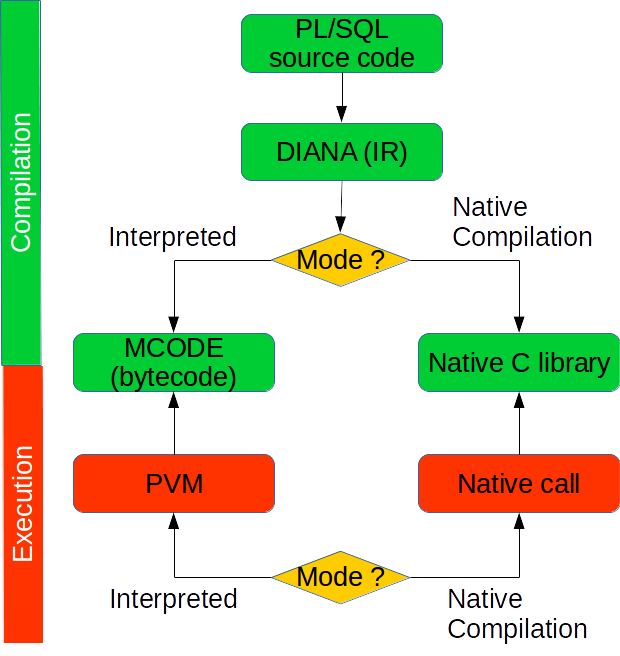
\includegraphics[width=7cm]{./graphs/CompilationModel.png}
	\caption{The compilation model of PL/SQL}
\end{figure}

\subsubsection{Native compilation}

To improve performance, it is possible, since Oracle 9.x, to compile the PL/SQL source program down to machine code, using the \textit{native compilation} option. This improves the performance of PL/SQL execution significantly, and can show 2x to 7x improvement over interpreted mode, depending on the input program. This is done by generating C code from the input program, then compiling this to machine code and linking it to the Oracle libraries.

This approach is still limited by some factors. First, to ensure correct semantics of the newly compiled programs, the generated code still has to perform shared library calls with the interpreter. These calls are expensive, and hard to optimize, even by modern compilers, due to the complexity of the whole system. Second, the improvement can only occur on the procedural section of the programs, as SQL statements in the program must still be sent to the SQL engine for execution. Due to the size of database tables, and the very fast speed of execution of native programs, these SQL statements really represent the bottleneck for such PL/SQL programs. Execution speed improvements are the most significant when the ran program does not contain any SQL queries, and is better for longer running programs.

In this project, we will try to improve performance over native compilation. We will focus on the use cases that already provides the best performance improvement in the native compilation case, for the same reasons. This means varying-length PL/SQL programs, called as UDFs in an SQL query. This ensures that we get significant performance improvements while still running typical PL/SQL workloads.

%\cleardoublepage
\startsection{The Graal / Truffle ecosystem}

This section gives insight into the environment used for this project, comprised of the Truffle framework and Graal VM.

\subsection{The Graal VM}

%\begin{itemize}
%\item virtualized objects through escape analysis
%\item Polyglot !
%\item find out more in the slides
%\item classes only loaded in interpreter mode
%\item re-use of the optimizations for all the implemented languages
%\end{itemize}

%\subsubsection{What is the Graal VM ?}

\subsubsection{A new JIT compiler for Java bytecode}

The GraalVM is an open-source project developped at Oracle Labs \cite{graalpage}. It is a high-performance Java Virtual Machine, using a very aggressive optimizing compiler, based on speculative runtime optimizations.

%It has been built with many goals in mind, more than being "just a new JVM".

Graal itself is a new compiler for Java bytecode. It is intended not only for Java programs, but for any programming language that targets this intermediate representation. The Graal VM is a complete Java Virtual Machine, that uses Graal as (one of) the JIT compilers. In GraalVM, the underlying virtual machine is the Hotspot JVM, but it is important to note that the Graal compiler is completely decoupled for its host VM. It complies with the JVMCI API (\textit{Java Virtual Machine Compiler Interface}), but assumes nothing about the virtual machine actually running the code. This allows the compiler to be used in various setups, which will prove useful when we talk about the SubstrateVM.

The compiler is entirely written in Java. This means that, when the JIT is triggered for the original program, the host JVM will interpret Graal's code. After some time, this code will get 'hot' as well, and be compiled dynamically. This compilation can either be done by Graal itself or by another dynamic compiler residing inside this virtual machine.

%The compiler is entirely written in Java. This means that the VM code can itself take advantage of runtime compilation and optimizations, as Graal is then dynamically compiled by the underlying JVM. In some instances, Graal can even compile its own code, and benefit from its own optimizations. To reduce the warmup time of the VM, some of its code is directly compiled when launching the VM.

%This means that any Java programmer can directly and simply access the compiler's interface. On top of that, this means that the VM can itself take advantage of runtime optimizations : Graal's code will be compiled at runtime by the underlying JVM. Graal even compiles some of its own code, which benefits from all its very aggressive optimizations. To reduce startup time of the VM, some of its code is directly compiled when launching the VM.

The major goal of the GraalVM is to provide very high-performance to high-level languages targeting the JVM, using speculative optimizations. To perform these optimizations, it uses its own GraalIR \cite{graalir, graalspecoptir}. This intermediate representation is graph-based, in SSA-form, and represents both control-flow constraints and data constraints. Nodes are only bound by their required constraints, meaning that some nodes may not have any control-flow constraint until scheduling occurs. This representation of the program makes the writing of optimizations much simpler than would be on a more classical IR.

% Some nodes of this graph can then be "floating", i.e. without any control-flow constraints, until scheduling occurs.
%This intermediate representation has been designed to facilitate the writing of optimizations.

%Some nodes of the graph can then be "floating", i.e. without any control-flow constraints, until scheduling occurs. This could be the case for a basic arithmetic operation for example, which only has data constraints on its operands.


\subsubsection{Speculative optimizations}

The dynamic compiler of the GraalVM makes extensive use of \textit{speculative optimizations}. Through tracing and profiling of the program's execution in the interpreter mode, the compiler is able to decide which branches of the program are very unlikely to be taken when executing in the compiled code.

Using this information, the compiler only produces code for the likely branch. This has two main advantages. First, the size of the compiled code is reduced. Second, this opens the door for many other optimizations. Indeed, the compiled portion of the code is only valid for a specific subset of inputs (the ones that satisfy the condition). This gives a lot of information about the possible types and values handled in that portion of code, which can be subject to virtual call elimination or partial evaluation.

The unlikely branch is not compiled, but instead replaced with a \textit{deoptimization point}. If such a point is reached during the execution of the compiled code, the execution must exit the compiled code, and continue running in the interpreter instead. For this to work, additional information must be stored in the compiled code to reflect the state of the interpreter at the deoptimization points. This information is later retrieved, and the interpreter can safely be started back from this point. The memory overhead of this technique has been looked at in \cite{graaldatacompression}.

Reaching a deoptimization point is expensive, because it means switching execution context, and continue running the rest of the code in the interpreter. Therefore, once deoptimization occurred, the compiler will typically re-compile with the branch that caused the deoptimization, to ensure it doesn't happens again.

The condition for deoptimization is called a \textit{guard}. It is handled like normal code in the IR, and thus can me moved in the program by the scheduler. They are typically moved out of loops, and checked as early as possible in the resulting compiled code, in order to minimize the impact of guards on performance.
%This makes the compiled code as fast as possible, by bothering it with checking guards only when and where it is totally necessary.

%Using speculative optimizations means that some optimistic assumptions made when producing the code will turn out to be wrong, sooner or later. This is why speculative compilers need to keep track of some information about the state of the interpreter, in the case of a deoptimization (i.e. when an assumption is found to be wrong). In fact, when runtime values break the assumptions made, the compiled code must continue in the interpreter. But the continued execution must not perform twice the same operation. That is why such compilers must store information about the state of the interpreter, in the compiled code or linked to the compiled code. Such overhead can be significant.

%The advantages of the GraalVM are mostly based on performance. Indeed, the heavy use of advanced and aggressive optimizations lead to increased performance over traditional JVMs (\todo{reference needed}).

%\begin{itemize}
%\item escape analysis
%\item example of speculative assumption : classes loaded now will be the only ones ! (abstract classes stuff)
%\item aggressive inlining
%\item trace-based jit
%\item use of profiling info
%\end{itemize}
%
%The integration of Truffle on top of the GraalVM also makes the latter interesting. Indeed, this allows for a relatively simple, yet high-performance way to implement a language. Truffle gives some information on the program being run (the guest language program) through profiling informations and the like, and the compiler produces very efficient code for it.
%
%For example, the compiler is able to make escape analysis further than it would otherwise. A value is found not to escape if it remains in the scope of a Truffle execution unit (called a \java{RootNode}). In this case, the value can be virtualized : no \java{Object} boxing is allocated for it, and all methods and fields can be accessed directly, without further indirection. This removes the overhead of allocating an object, and reduces GC pressure to perform garbage collection.
%
%Because the compiler assumes a lot of things to be constant, it can make more optimizations than traditional compilers. For example, Graal assumes that the set of classes currently loaded when the compilation starts will remain the same through execution of the compiled code. Because the code selected for JIT-compilation must have been executed multiple times before in interpreted mode, and because we know runtime-loading and replacing of classes is fairly uncommon, this is a reasonable assumption. However, for completeness, non-speculatives JVM cannot make such an assumption. Using this knowledge, Graal can perform inlining more aggressively, as a lot of classes, though not declared as \java{final}, do not have a subclass in the set of currently loaded classes.

\subsubsection{A multi-lingual platform}

Another goal for this project is to provide an efficient multi-lingual (or polyglot) platform. The idea is to share as much as possible the engineering intensive part of a virtual machine implementation across languages, in particular, the dynamic compiler that is crucial to performance.  Sharing the same runtime environment and dynamic compiler also make interoperability between languages easier  and more efficient. 
%The idea is to effortlessly be able to run multiple programming languages on the same virtual machine. This means cheap interoperability, because they all run in the same environment. This also allows every supported language to benefit from very complex optimizations, which would otherwise need to be re-implemented for every language.

To solve that open problem, the Graal team decided to bring all the languages to the JVM, while providing a simple way to integrate or re-implement the desired languages : the Truffle Framework. Efforts have also been made in order for the optimizations of Graal to take into account the fact that not all languages executed are necessarily Java at their core, and could use very different patterns.

\begin{figure}
	\centering
	\hspace*{2cm}
	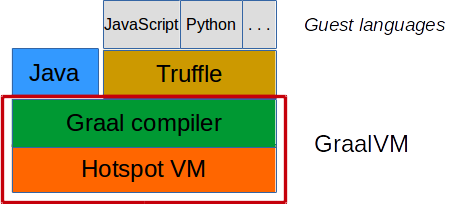
\includegraphics[scale=0.7]{./graphs/GraalVMStack.png}
	\caption{The complete GraalVM + Truffle stack}
	\label{fig:graalvmstack}
\end{figure}

\subsection{The Truffle framework}

\subsubsection{A language framework on top of Graal}

%\begin{itemize}
%\item runtime speculative optimization, through opt-deopt
%\item For more, see SL and cool tuto + actual doc (what is the link ?!?)
%\item polyglot environment, interop
%\item because compilation occurs at runtime, want to avoid a lot of re-compilations
%\end{itemize}

The Truffle framework is anoter open source project from Oracle Labs \cite{trufflerepo}, developped hand-in-hand with the GraalVM project. Its goal is to bring a variety of programming languages onto the JVM, so that they can benefit from the advanced optimizations implemented in Graal. Language implementations should be easy to write, and Truffle provides an API to write AST interpreters for this purpose.

We give in this section an overview of the features Truffle provides, focusing on the ones most important for this project. We will call \textit{guest language} a language that is running on the VM through the Truffle engine. The \textit{guest program} is the input program, written in the guest language.

%Support for additional guest languages must be added by programmers. Their task is to implement in Java the operators and semantics provided by the new language. Truffle provides an API to write AST interpreters, which are used to specify the guest language operations.

%The whole goal of the project is to limit the programmer's work to the implementation of such an AST interpreter, but still provide high-performance when executing the guest program. This is a real challenge, as the number of abstractions at play is large : the input program is run  by an AST interpreter, written in a high-level language (Java), running on the GraalVM, which itself runs on another JVM.

%To bridge that performance gap, 

%To do that, programmers must first re-implement the language's operators and semantics, in order to execute input programs of the \textit{guest language}. The guest language is the foreign language, not natively targeting the JVM, which is run by the Truffle engine.

%The Truffle framework is an open source project from Oracle Labs \cite{trufflerepo}, developped hand-in-hand with the GraalVM project. Its goal is to allow language designers or compiler / interpreter writers to get the same performance for some language implementation as a modern optimizer compiler machine code could produce, by only writing an AST interpreter. It does this by providing developers with a simple API, in Java, to describe the said AST. The interpreter itself then runs on the GraalVM, another project launched at Oracle Labs, and has many optimizations very specifically targetted towards this VM.

%The main advantage of the Truffle API is its simplicity and generality. It only asks that the language designer writes a set of AST nodes, extending some abstract class (with no abstract method), and uses a set of Java annotation to fetch some information from the nodes, and to ease the writing of the nodes themselves. An example of a simple  node for an imaginary language, using the Truffle DSL, is shown in Figure \ref{fig:truffleaddnode}.

%Under the hood, the Truffle framework also contains an annotation processor, which reads the interpreter code, fetches the relevant information, and automatically generates boiler-plate code for the classes written by the user. The fact that the code is duplicated allows for specific optimizations, but would be too much of a burden for a human to write and maintain. The fact that the process is automated \textit{removes} that tedious work from the programmer.

%The AST is not typed, and uses the fact that the class \java{Object} is a supertype of every value, including the primitive types through automatic wrapping (e.g. \java{int} to \java{Integer}). It would then be possible to write type-checks and type-casts inside the interpreter code to get the runtime value, and apply the operation. However, this method would both be lead to poor performance and low-quality code, requiring a lot of boxing / unboxing when dealing with primitive types. This is where specialization comes in.

\subsubsection{AST representation}

%\begin{enumerate}
%\item variables stored in the frame object, which can also be optimized out when functions are inlined
%\end{enumerate}

A common attribute to almost every programming language is the concept of expressions and statements. Using this, it is possible to represent every program of a certain language using an Abstract Syntax Tree (AST). If we want to execute such a program, we can use this AST form. Indeed, every node in the tree represents an operation, and its children supply the arguments to that operation.

Therefore, to execute a program in AST form, each node must do the following :
\begin{enumerate}
\item compute the values of the children nodes
\item execute the operation on the subvalues produced by the children
\item return the output value to the parent node
\end{enumerate}

%the children of a node must be executed first. Then, we can apply the operation to the produced sub-values, and return the output to the parent node.

Truffle provides an API to implement such AST interpreters. It also provides a DSL, based on Java annotations, useful for generating boiler-plate code. The representation used guarantees that almost every language can easily be implemented using this platform.

Each node in a Truffle AST must have a method called \java{execute}, which returns an \java{Object}. Nodes must declare their children using the \java{Child} annotation. Nodes also have a single parent, which is found automatically by Truffle when the tree is created.

Nodes can access and modify shared information, like variables states, through a \java{Frame} object passed during execution. Guest variables are then allocated on this frame object when the input program is parsed into the AST, meaning that the number and types of all the variables are known before running the program. Each guest variable must declare their storage type, which could be changed at runtime. This type is either a Java primitive type, or the generic \java{Object} type. This way, only the necessary space must be allocated, and primitive values need not be boxed.

%Such AST interpreters have been used for a very long time as a simple way to execute programs. However, their main problem is execution speed : for every node, we must find, at runtime, which operation it represents to be able to execute its code.

\subsubsection{The concept of specialization}

The concept of specialization is key in getting good performances from executing ASTs in the Truffle framework \cite{trufflespec, truffledsl}. It is a specific case of node rewriting.

In Truffle trees, nodes can be rewritten at runtime. This means that a specific node in the tree is replaced by another, typically with a more general implementation. In this case, the compiled code must be invalidated, thus requiring these events to be rare and stabilize during the execution of the program. This is useful when one wants to make an optimistic assumption on the input supplied to a node, and use a more efficient method of implementing the operation. If the assumption turns out to be false at runtime, the efficient implementation is replaced by a more general one.

This is exactly what happens in the case of specialization. It allows for an AST node to give multiple implementations for an operation. Instead of replacing the node completely every time, it only "activates" some of the implementation, which still acts as a node rewriting. The choice of which code to execute depends on guards, specified with the specialization, which check the input values provided to the node.

\begin{figure}[t]
	\lstinputlisting[style=Java, frame=single]{code/SpecializedAdd.java}
	\caption{Example of a simple Truffle node}
	\label{fig:truffleaddnode}
\end{figure}

Take the example shown in Figure \ref{fig:truffleaddnode}. It shows the implementation in Truffle of a simple "+" operator for a dynamically-typed language. In a simple implementation, the node would need to handle all cases. Instead, we can split the code, and add type-specific variants. Depending on the type of the inputs, Truffle will choose which code to execute at runtime.

Though nodes are simpler to write this way, this is not the only benefit from using specialization. Once a node has been executed, and one of its specialization taken, Truffle will make the assumption that every following execution of this node will take the same path. Only the guard for this specialization is checked, and everything else is replaced by a deoptimization point. This allows the node to be very fast for one specific set of inputs. If the assumption is invalidated at runtime, i.e. the guard is not satisfied for some input, then re-specialization is triggered. All the guards are checked for this input, and the specialization taken is added to the list of currently active specializations for this node. Only these two specializations are now checked at runtime.

If a node has too many active specializations, Truffle will deoptimize the node. The implementation will revert back to the general case, checking all specializations for applicability on every input. This is the slowest case of all, but the system is based on every node usually having the same kind of input during execution. Notice that like Graal, Truffle uses here a speculative optimization. In fact, this is eventually optimized out by the dynamic compiler. It will only compile the active specializations, and replace the others by a deoptimization point.

\begin{figure}[th]
	\centering
	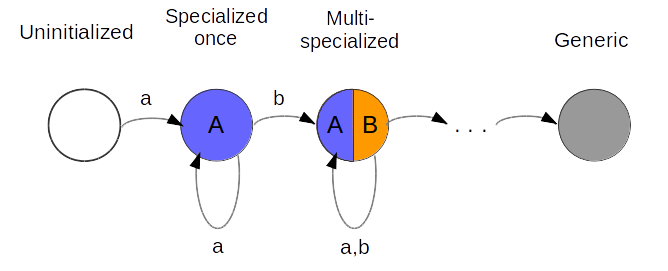
\includegraphics[width=12cm]{./graphs/SpecializationDFS.png}
	\caption{DFS representing the specialization process of a node}
	\label{fig:specdfs}
\end{figure}

The Truffle API allows for many ways to define specialization guards. The simplest one is to use the types of the input. The example used above shows such guards. Truffle automatically reads the signature of the declared specialization, and infers type guards for these. It will then execute the children of this node, and check their return type for a currently active specialization matching it, making type casts if necessary. It is also possible to write guards as a Java expression on the input values. Note that one can combine multiple types of guards to narrow down the specialization to a very specific case.

%The concept of specialization in Truffle is useful for many purposes, and solves the aforementioned problem, on top of opening plenty of very specific runtime optimization opportunities. Specialization is an annotation that can be added to a node's method, telling the Truffle API that this method is the implementation for the node, but only under certain conditions. Truffle allows specifying such guards in the following manners :
%\begin{itemize}
%\item Type guard : the said method is to be executed only if the input types match the method signature
%\item Expression guard : generic boolean condition that can depend on the input values
%\item Assumption guard : an assumption that is always assumed to hold, until an external events invalidates it
%\item Event guard : triggers re-specialization upon catching a specific kind of exception
%\end{itemize}
%
%When such an annotation is found, the annotation processor will generate a sub-node that contains all the boiler-plate code to make the checks and conversions, and call the correct specialization method. Note that mutliple condition-expressing variants can be used at the same time. It is also possible to have multiple specializations for which the conditions are satisfied at the same time. In this case, the current specialization, or first in the order of appearance in the node is taken. If no valid specialization is found, an exception is raised.
%
%Once a node's execution has completed, the specialized method that was executed becomes the current code for this node. On sub-sequent runs, the engine will only check the condition of the current specialization. If it does not match, then it will check all specialization again, as it did on the first run. The newly found specialization is added to the list of active specialization. On the following runs, both conditions will be checked, but no other.
%
%This multi-specialization phenomenon can only occur until a certain number of specializations is reached (this is an API constant). Once an input is found not to match any active specializations, and the maximum number of active specializations is reached for this node, then Truffle will stop trying to specialize this node, and test all possibilities on every run. \todo{add DFA showing specialization process}. This is useful to avoid re-compilations when the code has been \jitted{}.

%\todo{caches}

\subsubsection{Compiler primitive access}

As a high-performance framework, Truffle must provide programmers with very specific and fine-tuned tools to take advantage of the underlying compiler. The dynamic compiler in this case being Graal, additional profiling informations are very useful in order to help it make speculative assumptions and optimizations.

First, Truffle allows the specification of deoptimization points directly in the Java code. Any code following this instruction need not be compiled, as it must be executed in the interpreter. This is a simple way to make an explicit speculative assumption. It can be used to wrap very rare cases.

Truffle also provides a way to declare a value as being final while in the compiled code. This is again a speculative assumption, because such values need not be declared as \java{final} fields. This constant value can then be used for constant propagation and partial evaluation. On top of that, if the value is an \java{Object}, then Graal can inline the virtual calls as it knows the actual type of the value. If such values are to be changed during execution, then it is the programmer's duty to add a deoptimization point first. The compiled code is then invalidated, and will need to be recompiled later with the new value.

%The first, and most basic functionality a programmer could want is to be able to know or change the current execution environment. These methods can be found in the \java{CompilerDirective} class of the Truffle API, and allow the program writer to :
%\begin{itemize}
%\item exit a \jitted{} portion of code, returning back to the interpreter
%\item invalidate some already compiled code, requiring a new compilation later
%\item check whether the current code has been compiled or is being executed in the interpreter
%\item ensure that some portion of code is always executed in a specific mode (compiled or interpreted)
%\end{itemize}

%Alone, these functionalities may not be that useful when designing a tailored high-performance interpreter, as we would always like the code to be compiled. However, they are very useful when used in conjunction with another Truffle construct. One of the best examples of such use cases is the \java{CompilationFinal} annotation. It allows the programmer to specify that some value (typically the field of a class), even though it is not constant in the Java sense because it is not declared as \java{final}, will be a constant value when compilation occurs. To ensure that, the programmer needs to invalidate the compiled code whenever the value is changed. Upon JIT compilation, the compiler will treat this value as a constant, using its current value. This can lead to a lot of constant folding, partial evaluation and dead-code elimination if used correctly. Do note however that the annotated value should stabilize, other its changes would repeatedly trigger an expensive compilation.

%This is another measure to give more information about the program being run to the compiler. 

Truffle also lets the writer of the interpreter use explicit profiling. Profiles track information at runtime about values, in the form of simple conditions. For example, one could be interested in checking if the value of an input integer is always the same, or if the actual class of an \java{Object} value is identical for all runs. On top of profiling values (both the value and its type), it is possible to profile conditions and branches. Truffle provides specific profiling classes which can be used to check if an \java{if} branch is taken more than the other, or directly assume that a branch will never occur. These informations are then used by the compiler to make speculative assumption.

\subsection{High performance execution}

\subsubsection{Partial evaluation and inlining}
\label{sec:partialevaluation}

We have already seen, with specialization, that Truffle makes speculative assumptions (well understood by Graal) to improve performance. We present here another use-case, in the partial evaluation of executed ASTs.

Truffle makes the very simple assumption that the shape of the AST is fixed. Although not completely true because it provides support for replacing nodes in the tree on-the-fly, and that nodes rewrite do occur in the case of specialization, we can see that this is a reasonable assumption once the code has stabilized. Once the program is parsed, turned into an AST, and ran a couple of times (to give it time to stabilize), we can expect it to stay the same during the execution. With this very basic assumption, is is possible to reduce interpretive overhead significantly.

In Object-oriented languages, it is known that virtual calls are the source of many performance issues. This obviously happens here, as node execution is triggered by an abstract \java{execute} method call. However, because the assumption was made that the AST is constant once loaded, Graal can treat every node of the tree as a constant value. This means that it knows the actual type of all the nodes too. Using this information, it can then inline the \java{execute} calls in every parent node, starting from the root, to obtain a single and huge portion of Java code that represents the whole guet program. Optimization on such list of sequential instructions (not containing virtual calls) is rather easy. This aggressive inlining alone, is enough to remove the overhead of virtual dispatch when executing the AST.

This kind of optimization can be seen as a specific case of partial evaluation, in which the actual type of the receiver object of a virtual call is the constant value. That is why this very aggressive inlining process occurrs during the partial evaluation phase of the Graal compiler. In the general case, one would like to avoid inlining all of these functions, as that creates massive, monolithical fragments with duplicate code. However, this optimization is crucial to the performance of Truffle. For this reason, it is triggered only when compiling Truffle ASTs (other programs still benefit from regular inlining).

%We have seen that Truffle, as an API, provides very fine-grained tool support to tailor the performance of their interpreter, by giving more information to the underlying compiler. To pass this information to Graal, Truffle uses very clever mechanics, plus some internally built "communication" between the two.
%
%First, one can note that in the example shown in Figure \todo{reference needed}, the boiler-plate code generated also uses \java{CompilationFinal} annotations and constant flag masks to decide which specializations are currently active and skip guard evaluation for the inactive ones. Taken together, these seemingly simple techniques actually allow the Graal VM to know that all the inactive specializations are in fact, inactive, and that therefore, no code needs to be compiled for these. This is due to the fact that the \java{active} flag is constant during compilation for Graal. The current value is then \textbf{the} value for this field, and constant propagation makes all the inactive branches a '\java{if (false)}' check, which can be removed. Re-using its own primitives make the Truffle API both simple and very effective.
%
%Another example of such co-operation can be found in the AST interpreter's architecture itself. Indeed, because every node in the AST is a descendent of the same abstract class, a lot of virtual calls to the execute method of the subnodes are necessary. This would greatly degrade the performance, not only because such calls are expensive, but because they cannot be inlined, as the actual method implementation is unknown at compile-time. To solve this problem, sub-nodes in the Truffle AST must be denoted using a special \java{Child} annotation. The Truffle preprocessor, among other things, will add \java{CompilationFinal} annotation to these fields. Because the value is final while in compiled code, Graal can then inline all the calls, because it knows the runtime type of the subnode will always remain the same. This kind of tricks allow the Truffle and Graal framework to get performance close to native C implementations, as most of the high-level sugaring has been removed.
%
%However, one can see here that the \java{CompilationFinal} annotation, as well as the primitives contained in the \java{CompilerDirectives} class must bear a specific meaning for the Graal VM. It is indeed the case, as Graal is coded with some knowledge about Truffle, making it the only viable VM to use Truffle on. This requirement is somewhat lifted, as the Graal VM is also implemented in Java, and can then be run on any classic JVM.

\subsubsection{Boxing elimination}

Another major performance issue with this kind of interpreters is the overhead of boxing primitives values.

Because the return type of a node cannot be statically determined, values produced are passed as generic \java{Objects}. When passing primitive values, this means allocating a boxed object for it, then unboxing it at the use location to perform the operation on the value itself. The result is then wrapped, yet again, into an \java{Object} box, before being returned to the caller. This adds a lot of runtime overhead. On top of that, if a lot of such boxes are allocated, then repeated execution of the garbage collector can cause massive slowdowns as well.

To solve this issue, primitive values should not be boxed at all. The first way Truffle can avoid these is very simple : add static type information in the Java interpreter's code. To do that, one can add type-specific \java{execute} methods to their hierarchy of nodes. When relevant, the caller can then apply the correct method, and be ensured of the return type, removing the need for a box to be allocated. An example of such a use case is shown in Figure \ref{fig:truffleifnode}. If the called node cannot supply a value of the expected type, then it must throw a specific caught exception, which contains the generic value as an \java{Object}. The caller is then responsible for handling this exception and its value.


\begin{figure}[t]

	\begin{subfigure}[h]{\textwidth}
		\lstinputlisting[style=Java, frame=l]{code/Node.java}
		\caption{Abstract node defining the typed execute variants}
	\end{subfigure}
	
	\begin{subfigure}[h]{\textwidth}
		\lstinputlisting[style=Java, frame=l]{code/UnboxedIf.java}
		\caption{'If' node using typed execute}
	\end{subfigure}
	
	\caption{Example of typed execute usage}
	\label{fig:truffleifnode}
\end{figure}


Another way to eliminate boxing is by using an automated way. Graal implements that, by performing an escape analysis phase. The goal of this analysis is to figure out if some value can escape its local context, and be used as a generic object somewhere. If a primitive value is found to escape, then the box must be allocated, otherwise some foreign access could be invalid. If the value is proved to stay local only, then the primitive value can be accessed directly in all use sites, and no box is created. Though this optimization can be hard to carry out in the classic AST form, it is much simpler when performed on the completely inlined version of the same tree, as discussed in \ref{sec:partialevaluation}. In this case, the scope for the escape analysis is the local code block, e.g. loop body or condition branch, or the Truffle program itself (the whole tree, starting at the root).

Using the exact same analysis and concept, it is possible for Graal to avoid the allocation of other objects, not only boxes around primitives types. If a class is instantiated, and the newly created value is found not to escape the local context, then allocation can be avoided. The fields of the object are replaced with local variables, and access to the fields are made directly on these values. In this case, the object is said to be \textit{virtualized}.

With this, allocation for most of the local values can be eliminated. In fact, most values remain local to the program only, and are never visible outside. Notable exceptions are values used as arguments for function calls in the guest language, return values of guest language functions, and values stored in another objects' field.

\subsubsection{Example}

We present here a small example of an interpreter's run using Graal and Truffle, to explicit the concepts described. We use a language with a single node, presented in Figure \ref{fig:truffleaddnode}, which performs a "+" operator for a dynamically typed language. It performs an addition on numeric inputs, and concatenation for strings. We also consider the very simple program "$a + b + c + d$", whose corresponding AST is shown in Figure \ref{fig:astadd}. We will show that even with simple interpreter code written in a high-level language, it is possible to get close to the optimal machine code we would expect.

\begin{figure}[thb]
	\centering
	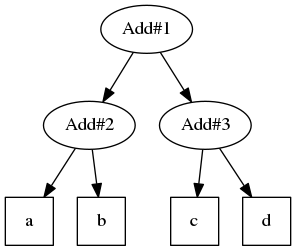
\includegraphics[width=5cm]{./graphs/astadd.png}
	\caption{AST for a simple input program}
	\label{fig:astadd}
\end{figure}

%For the sake of this example, say the values $a$, $b$, $c$ and $d$ are always integer values. In this case, the basic interpreter would do a lot of additional work compared to the simplest machine code we would like to get for this program :
%\begin{itemize}
%\item virtual calls to the sub-nodes \java{execute} method
%\item boxing of primitive values (\java{int} in this case)
%\item type checks on the values' runtime type
%\item type cast and unboxing of the primitive value
%\end{itemize}
%
%This additional work must be done by every node in the AST. We show that the framework is able to eliminate all of this, and produce the machine code we would expect from this program.

For the sake of this example, say the values $a$, $b$, $c$ and $d$ are always integer values. In the first run, the nodes 2 and 3 specialize for the integer type, and so does node 1. This means that Truffle now makes the assumption that the inputs will always be of type integer, and only check for this condition.

After a certain number of run, the JIT compiler will trigger. Reusing the assumptions made by Truffle, it will make speculative optimizations on the inputs being of type integer. Only the integer addition code for the nodes needs to be compiled. A guard is added to check that the input are indeed of type integer, and a deoptimization point set in the invalidating case.

As we said earlier, Truffle also makes the additional assumption that the tree does not change. Once again, using this assumption, the compiler is able to inline the code of the whole tree, starting at the root node. It can now remove the guards in the code for node 1, because the only possible output of nodes 2 and 3 are integer values. Boxes can also be eliminated after escape analysis, and replaced with uses of \java{int} values.

What remains after these optimizations is a code that does the following :
\begin{enumerate}
\itemsep0em
\item load the values for $a$, $b$, $c$ and $d$
\item check that they are of type \java{Integer}
	\begin{itemize}
	\vspace{-1mm}
	\itemsep0em
	\item if not, deoptimize
	\end{itemize}
	\vspace{-1mm}
\item unbox the values
\item perform addition on primitive integers
\end{enumerate}

We can see here that the code is not completely as we could expect. Some guards still remain, but need to be for correctness. Because we have no knowledge about the way the values are loaded, they are loaded generically, and need to be unboxed. Note that this could be optimized away, depending on the nodes used to load these values. But the cost of boxing / unboxing is removed for the root node, and arithmetic add operations are performed sequentially without any additional checks.

\begin{figure}[t]
	\centering
	\makebox[\textwidth]{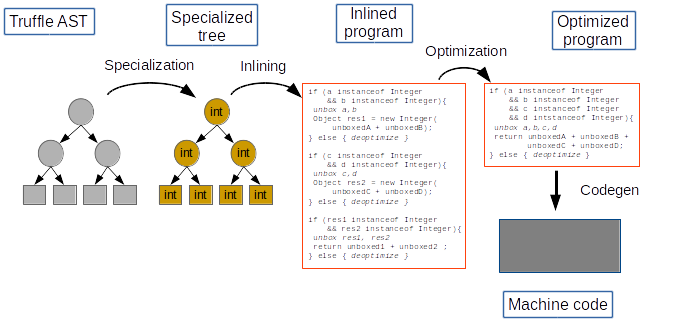
\includegraphics[width=15cm]{./graphs/VisualExample.png}}
	\caption{The steps taken by the interpreter code before it becomes highly-optimized machine code}
	\label{fig:visualex}
\end{figure}

Finally, let us consider the case where, after the code has been compiled in the way described above, some guards become invalid. For this example, we will assume the values suddenly become \java{String} values. In this case, the guards of nodes 2 and 3 are invalidated. This triggers deoptimization, and Truffle must re-specialize the said nodes. From now on, guards for \java{Integer} and \java{String} must be checked. The same then occurs for node 1.

Once this new tree has been run many times, a new compilation will occur. But the room for optimization is now smaller, as less is known about the values in the program (they could either be integer values or strings). The code will be less performant, and need to take the decision on whether to add or concatenate at runtime. However, this case is assumed to be somewhat infrequent, even in untyped languages, because a single node in the AST will usually treat the same types.

%For JIT-compilation to occur, the nodes must have been run a fair number of times first. As we said, only integer values are supplied at the leaves of the AST. This means that the 3 \java{Add} nodes are specialized for the input type \java{int}. Information about specializations is stored in \java{CompilationFinal} fields in the nodes, and uses comparisons with constant flags to check which specializations are currently active, and thus which guards need to be checked. Performing a simple constant folding optimization, Graal can easily find out that all the inactive specializations can never trigger during the compiled code's execution. It can therefore remove all the code for this, and keep only the type guards and addition's code for integer arguments.
%
%For each AST node, sub-nodes are declared as being \java{CompilationFinal} as well. Therefore, Graal knows the exact type of each sub-node, and can easily inline the calls to the \java{execute} method. As it is only comprised of a type check for \java{Integer} values, plus a basic "$+$" operation, many optimizations can be carried out. First, the return type is always known. It is not generic anymore, and is known to produce only integer values. Therefore, the type check in node 1 can be removed. This also means that boxing can be removed. In the end, only the raw addition operator on simple Java integers remain, which is what we expect. This code is then natively compiled, and produces very efficient machine code compared to the high-level interpreter we wrote.
%
%Now, as a final note, let us the consider the case when the said code has been compiled, and guards break. Say for example that $c$ and $d$ produce a \java{String} value. In this case, the input guard of the lower \java{Add} node number 3 does not hold anymore. Code is deoptimized, and execution is continued in the interpreter. The concatenation specialization is added to the list of active specializations, and execution continues. When JIT-compilation will trigger next time, both specializations will still be active. Less optimizations opportunities will be available in this scenario. However, we can expect a single AST node to get the same kind of input values at runtime, even in an untyped scenario. It is this assumption that gives very good performance to untyped languages on the Truffle/Graal engine.

\subsection{SubstrateVM}

\subsubsection{An embeddable VM}

Although the GraalVM does provide very good performance to Java and foreign languages programs, it does have some limitations. Java Virtual Machines in general are known to have high memory consumptions, and long warmup times. These problems are not acceptable when the goal is to integrate Graal and Truffle inside another system.

To be able to integrate the Graal compiler and the languages implemented with Truffle that run on top of it, the Graal team implemented a new way to execute them : the SubstrateVM (abbreviated SVM). The Substrate VM is a very thin virtual machine that provides the necessary services to run Truffle interpreters. It provides a garbage collector, thread support, and works with most of the JDK library. Its main goal is embeddability, so it should have a very low warmup time and a small memory footprint.

To be embeddable, the SubstrateVM should be self-contained, which means that runtime class-loading is not possible. Further, the SVM is not a JVM, and does not behave like one. Thus, some low-level calls or virtual machine specific knwoledge cannot be used here, like reflection for example. These restrictions form a subset of the Java language, feasible for SVM integration. Sources to be deployed on SVM, as well as any reachable code, must be written in this subset and comply to the restrictions.

\subsubsection{A pre-compiled VM}

The GraalVM, due to its complex and highly-layered structure, has very long warmup times. When executing a guest language program, multiple artifacts must be compiled before the executed program reaches peak performance :
\begin{enumerate}
\item the underlying JVM must get to warmup, and start compiling Graal's code
\item Graal itself must warm up, and start compiling the interpreter code
\item the nodes of the AST interpreter must stabilize for the inputs seen, and stop any deoptimization : this is the optimal code
\end{enumerate}

To solve this issue, the SVM is built as an already compiled entity. This way, the only compilations that take place at runtime are guest language program compilations.

The Substrate VM is also implemented in Java. To build a pre-compiled image, multiple steps are required. First, the relevant sections of code must be found. This include SVM and Graal's code, on top of the desired Truffle interpreters, and any library these may use. This is done by performing static reachability analysis, starting from these pre-defined components. The analysis is performed by Graal, which has dedicated modules for static analysis. Once these classes and methods are found, they will be the only ones available in the image. This is due to the requirement of SVM being thin and slef-contained, and removes the burden of checking for and loading missing classes at runtime.

After that, the code is compiled ahead-of-time using Graal. As we said earlier, Graal is not bound to be a JIT compiler in a specific VM, and can be used in many contexts. This is one of them, where it is used as an ahead-of-time Java bytecode to machine code compiler. The resulting image is rather small, as it contains only the necessary parts of the code, with a size between 200 and 250 Mb for the PL/SQL images we built.

%The idea of the SubstrateVM (SVM for short) is to create a pre-compiled image of the GraalVM. This image should be self-contained, i.e. not requiring loading any other classes at runtime. The goal is to reach peak performance faster, by spending all the time executing the guest program, and not compiling the VM.

%Static analysis must be performed to know which code to embed in the compiled image. SVM must act as a JVM when running, so it has its own garbage collector. The code is compiled using the Graal compiler itself, but can only perform static optimizations (although specific care is taken when compiling Graal's own code).

The guest program, because it is represented as an AST in memory and loaded at runtime, can only be compiled dynamically. As we showed earlier, this is desirable to benefit from speculative assumptions. This means that runtime compilation can still occur in the SubstrateVM, but it is limited to Truffle programs. To be able to do this, the image must carry specific information about the code that is susceptible to just-in-time compilation. This includes the code of the interpreter's nodes themselves, but also the parts of the Truffle API used by the latter, and generally any code reachable from the AST nodes. It is possible to restrict this set, by 'hiding' some code behind specific Truffle boundaries, provided by the DSL. This can avoid loading massive portions of code from external libraries, which may not benefit a lot from dynamic compilation. Because the complete environment is statically-compiled, warmup times for the guest program are typically very short. The compilation time overhead can be reduced by performing compilation on a separate thread.

%\subsubsection{The problem of warmup}
%
%Despite its advantages, the Graal VM can have problems with warmup times. Because it is written in Java, and runs on another JVM, multiple layers of JIT compilation and warmup must occur before optimal performance is reached :
%\begin{enumerate}
%\item the underlying JVM must get to warmup, and start compiling Graal's code
%\item Graal itself must warm up, and start compiling the interpreter code
%\item the nodes of the AST interpreter must stabilize for the inputs seen, and stop any deoptimization : this is the optimal code
%\end{enumerate}

%Note that this does not incur a cost if the execution was taking place in the interpreter, because no time has been spent (and wasted) in compilation of this later discarded code. Due to this time required for the nodes to stabilize, the JIT compiler should wait for a fair amount of time before deeming some code as "hot", to avoid wasteful compilations. However, once the code has been compiled and run a lot of times, it is still possible that some unexpected input appears and requires re-specialization of some node(s). After that point, compilation should be very fast.

%The third point here is very important for the tuning of Graal. While specializing, the guest program AST will need to invalidate the currently compiled code. Truffle provides some measurement of stability of the tree to avoid such deoptimizations, but cannot be guaranteed to never occur later. On top of that, this means waiting a fair amount of time for very simple programs before the code gets compiled.

%Unfortunately, this problem is hard to solve, and leads to long warmup times for programs running on the Truffle/Graal engine. The goal being to reach peak performance as soon as possible to reap the most benefits, this approach is not suitable. That is why the Graal team created a new way to use their VM, with lower memory footprint (running two JVM inside another requires a lot of memory) and faster warmup times. This is the tool of choice for embedded integration and benchmarking, and is called SVM.

%\subsubsection{The SubstraveVM}
%
%The idea of the SubstrateVM (SVM for short) is to create a pre-compiled image of the GraalVM. This image should be self-contained, i.e. not requiring loading any other classes at runtime. The goal is to reach peak performance faster, by spending all the time executing the guest program, and not compiling the VM.
%
%Static analysis must be performed to know which code to embed in the compiled image. SVM must act as a JVM when running, so it has its own garbage collector. The code is compiled using the Graal compiler itself, but can only perform static optimizations (although specific care is taken when compiling Graal's own code).
%
%The guest program, because it is represented as an AST in memory and loaded at runtime, can only be compiled dynamically. As we showed earlier, this is desirable to benefit from speculative assumptions. The compilation time overhead can be reduced greatly by performing compilation on a separate thread.

%Due to the heavy-weight static analysis and optimizations that must be performed, generation of the SVM image is rather slow. However, it is built to provide very good runtime performances, so time lost in building the image will eventually be compensated by the improved running time. On top of that, the SubstrateVM has been designed for very specific purposes which do not take into account the compilation time (integration and performance measurement for example).

\subsubsection{Direct C access}

Easy and efficient manipulation of native C types and data structures is key to embedding languages in complex host systems. The Java virtual machine provides an interface that can be used to interact with external code and values, namely JNI (for \textit{Java Native Interface}). This solution is hard to use in practice, as writing such code is cumbersome and has poor performances. The SubstrateVM offers specific abstractions to ease the interactions between Java and C code, and does so in a lightweight fashion.

%On top of being faster, and with a lower memory footprint, the SubstrateVM provides a few additional tools. The most important of these is a very efficient access to C structures and code.

Because SVM is compiled natively to machine code, and is not bound by the restrictions of a JVM, it is possible to make easy and very efficient direct memory accesses. The Substrate VM uses this to provide fast interfacing with external C code and structures. It supports the C primitive types without any conversions in Java, as well as pointer arithmetics. It allows C data structure access and function calls to and from C.

SubstrateVM provides a DSL to declare the C structures used in the Java code, which are then used as Java \java{interface}s. When compiling the image, the Java access methods are replaced with direct memory accesses into the C data structures. This \java{interface}-based mechanism allows the Java code to be clear, type safe, and valid for compilation by any Java compiler.

The DSL also provides mechanisms for function calls, to and from C. Java methods to be called from C should be \java{static}, and never called inside the Java codebase. Some annotations must then be added to its declaration to make it accessible. The function can then be called in C using function pointers. Java code can also call C functions easily, by providing the name of the target entity. These calls are resolved when linking the image.

%For type safety in the Java code, the C structures used must be "re-declared" in Java, using DSL based on annotations that SVM provides. C structures can then used as Java \java{interface}s, and these accesses are replaced with direct structure access during image compilation.

%Because the SVM is an entity of its own, it is not bound by the JVM's limitations like Graal is. Indeed, Graal VM being run in another Java virtual machine, it cannot easily make very low-level calls or accesses to the memory, and is bound to the memory-safe environment of Java. The SVM, as it is compiled directly to machine code, lifts these restrictions, and permits direct access to memory. 

%All the C structures, types and methods can be accessed directly form Java. No conversions are performed between Java and C primitive types. For type safety in the Java code, the C structures used must be "re-declared" in the Java code, using another DSL based on annotations. After that, all calls and structure access, as well as pointers arithmetics are available. Note that this works both ways, and allows the C code to call Java functions as well, through C function pointers.

This is very useful when interacting with lower-level APIs, and allows fast and efficient interoperability. We use these functionalities in the project to get direct access to the values provided by the database, without requiring a copy into the Java heap.

%\cleardoublepage
\startsection{Implementing a subset of PL/SQL using Truffle}
%\thispagestyle{plain}

We describe here our approach for implementing a subset of PL/SQL using Truffle. It uses all the tools provided by the framework to achieve high-performance. It also exploits the static typing of PL/SQL to implement improvements based on data representation specialization.

%\begin{itemize}
%\item we talk in this section only about integer types
%\item remember \plsi{} and \simpleint{} differ in null and overflow semantics
%\end{itemize}

\subsection{Naive approach}

%\begin{itemize}
%\item Truffle designed for dynamic languages (proof : most paper on JS)
%\item static typing helps specialization because only one type will actually appears at run time
%\item data types used to specify which semantics. can be used for more, like representing subset of values
%\item example of naive implementation
%\item explicit boxing
%\item values carry the information on null
%\item \maybe{can do a lot of optimizations on the given example (branch profiling, specializations on left or right being null ...), but still has problem}
%\end{itemize}

We first present a simple approach to building an interpreter for PL/SQL, based on how dynamic languages are typically implement within the Truffle framework.

In this system, basic operators (e.g. "$+$", "$-$", "$<$") are represented by a single node which can handle every input. It declares specializations for the valid pairs of type that the operation can be performed on, and defines the semantics of the operation in this case. An example of such a node is given in Figure \ref{fig:naiveadd}.

\begin{figure}[t]
	\lstinputlisting[style=Java, frame=l]{code/NaiveAdd.java}
	\caption{Naive add implementation for PL/SQL}
	\label{fig:naiveadd}
\end{figure}

For this system to work, every type in the guest language (PL/SQL in this case) must have a corresponding, and unique, Java type to represent it. Values of the guest language can only be represented by these types. We therefore have to find a mapping between PL/SQL types and Java types. A natural way to do so is to create a class for every type, and box all required information inside.

We would like to use Java primitives types when possible for such mappings. \simpleint{} naturally maps to \java{int}, but \plsi{} cannot map to the same Java type. Being a nulleable type, values of the type \plsi{} need additional information to represent the possibility of a value being \plsnull{}. A simple solution is to create a class for this type, comprised of a 32-bit integer value and a flag for \plsnull{}.

However, this solution incurs a lot of overhead on boxing and unboxing, and increases memory consumption. For operations on non-null values, the integer value is unboxed, the operation is performed, and the result is the boxed again in a new object. For null values, the flag must be checked, but no object needs to be allocated : the null value found can be reused. We expect values to be non-null most of the time, which has the highest cost. Note that Graal should be able to virtualize most of these object allocations. This would make us very reliant on Graal correctly performing its escape analysis, and suffer a heavy cost when some value appears to escape.

\subsection{\plsi{} and \plsnull{} handling}

%\begin{itemize}
%\item in dynamic languages, or naive approach, specializations determine semantics
%\item here static info determines semantics, specializations handle a specific representation
%\item specialization on type representation rather than operation implementation
%\item mostly make use of type guards and specialization, as each type representation has its own type (but a single java type can be used by multiple pls types)
%\item java types can now represent an in-memory representation
%\item can make assumptions that only single data rep will be used at a specific location (same principle as same type for specific node in JS)
%\item values can still be boxed when passed as generic values (return value, argument passing)
%	\begin{itemize}
%	\item reduced when guest functions are inlined
%	\item naive approach was using explicit boxing (might be harder to optimize by Graal, but still done through escape analysis)
%	\item if so, objects are virtualized \maybe{add to graal presentation}
%	\end{itemize}
%\item most operations all the same for null value, simpler to write this way
%\item all nodes not re-implemented : only those who need to apply different semantics do. generic value sinks (write, read ...) need not. type information kept in the nodes tho.
%\item null check made cheaper by reference comparison
%\end{itemize}

To alleviate this problem, we would like to be able to use primitive \java{int} values to represent non-null \plsi{} values, and a specific \plsnull{} value otherwise. However, this cannot work in the system described. Because the operators choose semantics using the input Java type, they cannot differentiate between \plsi{} and \simpleint{}, which have different semantics on overflow (the first raises an exception while the other does nothing). This is the typical implementation of dynamic languages in Truffle, where the input type defines the semantics used.

We use the fact that PL/SQL is a statically-typed language to fix these issues. Using type information from PL/SQL, we build a statically-typed AST. Every node can only handle values of their fixed type. We can then safely map different PL/SQL types to the same Java type. In this system, we can also use different Java representations for the same PL/SQL type. This will be the basis for data representation specialization.

\begin{figure}[p]
	\centering
	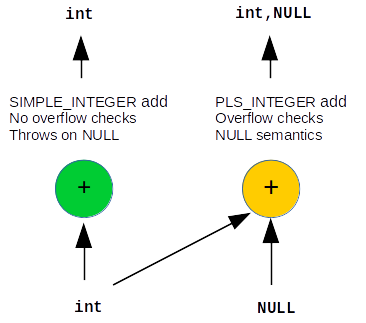
\includegraphics[scale=0.8]{./graphs/TypedNodeExample.png}
	\caption{Statically-typed AST nodes for addition}
	\label{fig:typednodeexample}
\end{figure}

Both non-null values for \plsi{} and \simpleint{} use the primitive integer type. Further, we add a specific type to represent the \plsnull{} value, implemented as a singleton. Specializations in the operation nodes can now be performed on primitives types when possible, reducing the stress for escape analysis and boxing elimination.

\begin{figure}[p]
	\lstinputlisting[style=Java, frame=l]{code/PlsIntegerAdd.java}
	\caption{Code of a statically-typed add node for \plsi{} values}
	\label{fig:plsiadd}
\end{figure}

This system is aimed at helping Graal produce more optimized code. First, removing explicit boxing lightens the dependency we can have on Graal effectively escape-analyzing all the values, and virtualizing the corresponding objects. On top of that, Graal understands more easily the primitive types and their respective boxes than hand-crafted re-boxing. Note also that type information is easier to propagate for the compiler than flag values in an object's field. This helps partial evaluation and constant folding, especially concerning type guards in Truffle specializations.

Finally, this solution replaces typed null values with an untyped generic \plsnull{} value. This makes the writing of nodes and conditions simpler, and requires less checks. However, this also requires writing one node per type and per operation. Although this can seem tedious, the Truffle DSL helps greatly in reducing the amount of work required, and reduces the number of possible specializations for each node. This duplication is only limited to semantics-based operators, some other nodes need not care about the type (e.g. write, read).

\subsection{Storage model}

%\begin{itemize}
%\item storage model
%	\begin{itemize}
%	\item variables stored on the \java{Frame}
%	\item different values stored (int and null) require Object frame slot
%	\item means boxing again
%	\item solved by adding a simple boolean field for null values
%	\item kind of specific optimization, but null present almost all the time
%	\item easy to optimize out if boolean value never changed (constant propagation)
%	\item otherwise, added check on every frame read (should be lower cost than unboxing on every read)
%	\item not null constraint checked, and memory + runtime overhead removed when value cannot be null
%	\item \maybe{note: guest variables understood by Graal as native variables through virtualization of the array (frame variable only local to the guest function)}
%	\end{itemize}
%\end{itemize}

To represent program state, PL/SQL uses typed variables. Program variables in Truffle are stored in a specific object called the \java{Frame}, and passed along during execution of the nodes. Values must be stored in pre-allocated slots in the frame. These \java{FrameSlot}s must know about the type of value that will be stored : either primitive, e.g. \java{int}, \java{boolean}, or the generic \java{Object} case. They do not store information about the actual type of objects stored, but type profiling could be added when reading from the frame.

The typing of the frame slots poses a major problem for the system we described. Indeed, if a \plsi{} value is stored, the type of the frame slot should depend on the actual value : \java{Object} slot for the \plsnull{} value, \java{int} slot for the others. Because compilation optimizations depend on the types of the frame slots, changing it causes deoptimization.

One solution would be to optimistically use integer slots until a \plsnull{} value is found. This event would trigger deoptimization, and switch the slot to a generic \java{Object} one, able to store both the singleton null value and integer values. This is called \textit{frame slot specialization}, and is used in the Truffle implementation of Javascript for example. However, this means that non-null values must now be boxed when stored. This boxing is not escape analyzed by Graal (because the object is stored on the frame), and leads to huge overheads in allocation and garbage collection times.

We use a very simple flag based system to solve this. Nulleable variables are reserved two frame slots: one for the value if non-null, the other for a \java{boolean} indicating whether the value is \plsnull{}. This flag is first checked before returning either the null value, or the actual value stored in the other frame slot. This removes boxing, but adds another runtime overhead (added check when reading) and memory overhead (two frame slots per variable).

Though minimal, these overheads can be removed for variables that cannot be null. PL/SQL defines a \pls{NOT NULL} constraint, which ensures that variables cannot be \plsnull{}. Some types, like \simpleint{}, are \pls{NOT NULL} by default. For these variables, we can remove the second frame slot and the added check.

\subsection{Language support}

%\begin{itemize}
%\item what we implement
%	\begin{itemize}
%	\item which operators
%	\item builtin calls
%	\item function calls, even though not tested in the database integration (comparison meaningless)
%	\end{itemize}
%\end{itemize}

For this interpreter, we implemented a subset of the PL/SQL language. This subset is enough to express most programs, but does not contain any of the builtin support for SQL. For more details on the operators listed here, please refer to the PL/SQL documentation \cite{plsdoc}.

We support most of the control flow operators that PL/SQL provides. This includes conditional branching (\pls{IF}, \pls{CASE}), loops (\pls{WHILE}, \pls{FOR}, unconditional \pls{LOOP}), loop-specific control flow (\pls{EXIT}, \pls{CONTINUE}) and return statements (\pls{RETURN}, with and without a value). The only control flow we do not support are direct branching (\pls{GOTO}) and cursor-based operators (\pls{FORALL}).

For defining programs, we support top-level standalone \pls{FUNCTION}s and \pls{PROCEDURE}s. A PL/SQL procedure is simply a function that does not have a return value. They are usually used for stored procedures.

The types we support in our interpreter are the integer types \plsi{} and \simpleint{}, plus the string type \varchar{} (detailed in the next section). As explained above, we provide full support for the \plsnull{} semantics of PL/SQL. \pls{NOT NULL} variables are also supported, and slightly optimized as explained above. Incomplete supports for \pls{BOOLEAN} and \pls{NUMBER} have been added, but should be looked at as future work.

We implemented the basic operators for every type supported. This includes arithmetic operators on integers (\pls{+}, \pls{-}, \pls{/} and \pls{*}), concatenation on \varchar{} (\pls{||}) and logical operators on booleans (\pls{AND}, \pls{OR} and \pls{NOT}). We also have comparisons ($=$, $!=$,$<$, $>$, $\leq$, $\geq$, \pls{IS NULL}, \pls{IS NOT NULL}), which work on every type.

Finally, to increase the expressiveness of our subset, we added support for builtin function calls, and provide an extensible framework to allow the simple and incremental addition of new builtin nodes. Some numeric builtins are supported (\pls{ABS}), and more \varchar{} builtins (\pls{LENGTH}, \pls{SUBSTR}, \pls{REPLACE}), as this is the only way to handle and modify \varchar{} values.

We believe this is a subset of enough importance to allow writing meaningful programs. We will test this hypothesis when building micro-benchmarks in section \ref{sec:benchmarks}.

\subsection{Compilation model}
%\maybe{should this be moved to a separate "database integration" section ?}

We present here briefly how we compile PL/SQL programs to Truffle ASTs before executing them.

The PL/SQL compiler already provides a way to generate an AST from the source programs. As explained in section \ref{sec:plscompilation}, the first pass in the compiler is to build a DIANA representation of the program. This DIANA form is effectively a typed AST for the compiled program.

To build the Truffle AST, we let the normal compilation process start, and intercept the DIANA tree once it is complete and annotated with type information. We then store it in JSon format to make the parsing easier. This extraction is only performed when the user activated our replacement interpreter, which is done through a system parameter. Note that we aim for non-disruptive incremental changes to the basic PL/SQL execution environment. Therefore, once we extracted the AST, we let the normal compilation continue, as a fallback if the user wants to execute with the classic engine.

\begin{figure}[tb]
	\centering
	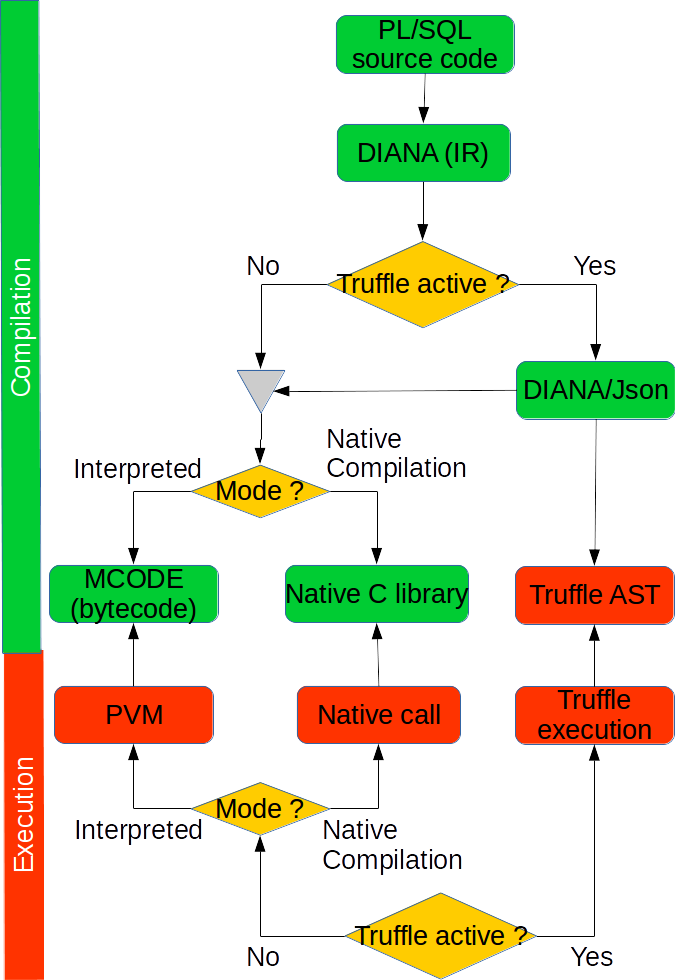
\includegraphics[width=8cm]{./graphs/CompilationModelExtended.png}
	\label{fig:compmodelext}
	\caption{The new compilation model for PL/SQL, with the addition of our Truffle interpreter}
\end{figure}

JSon programs are parsed on the first execution of the program. From the AST, we generate one Truffle node for almost every DIANA node. We also gather information about the types and variables used. Whenever an operator node is found, we analyze the type of the expression to use the correct statically-typed Truffle node, as discussed when explaining the design.

This solution for compilation is simple and reuses already existing tools.

%To produce the abstract syntax tree from the source PL/SQL program, we make use of the existing system and tools. As previously explained, PL/SQL sources are represented as DIANA in the first pass of the compiler. This is tree based, and effectively represents an AST for the input program. We 

%\subsection{Type system in the interpreter / Type representation and runtime specialization of representation}
%One PL/SQL type to multiple Java types in the interpreter (multiple representations for most types)
%\subsection{Runtime type-specialization}
%Possible to use base, raw types because language is statically typed (ex: PLS\_INT overflow semantics)
%\subsection{Null handling}
%\begin{itemize}
%\item Unboxed
%\item Using only base, raw types for nullable int
%\item No need for additional boxing when handling plsinteger
%\item Type-specific nodes, so no need for specializing on input type for choice of semantics
%\end{itemize}

%\cleardoublepage
\startsection{Efficiently implementing VARCHAR2}
\label{sec:varcharimpl}

We describe in this section the design decisions we took for implementing the \varchar{} type. We extend on the concept of data representation specialization to improve performance.

%\begin{itemize}
%\item reminder to go back to section .. ?
%\item different charsets not supported
%\item multiple charsets not supported
%\item assumption made that usually, the representation of a value when it arrives at a node is always the same (always follows the same route / same sequence of operations)
%\item conclusion : while simple, string implementation still shows improvement over naive approach. further work could be done to improve over the current solution.
%\item we use string denomination for varchar as well
%\end{itemize}

%Future work :
%\begin{itemize}
%\item future work : loop unrolling
%\item point to ways of reducing the polymorphism (type hints, like \# of each kind)
%\item with the system, can also add ropes for example, or a specific type for replace if becomes bottleneck
%\item could profile the actual type of the list to see what's up
%\end{itemize}

\subsection{Design constraints}

%\begin{itemize}
%\item should provide very efficient concat operator (copy less if possible)
%\item can change representation transparently
%\item code should all be inlined, need to know the actual type at all times
%\item avoid virtual calls when possible
%\item must specifiy the data type or cast all the time
%\item should handle all variants at all times as well
%\item need not re-copy the code if wrapped in type-safe stuff
%\item most operations are concat of short strings, but also processing of very long ones (need to benchmark both worloads)
%\item explain what the string building workload is
%\end{itemize}

The \varchar{} type of PL/SQL has many specificities.

First, there is no direct access possible to the underlying representation of such values. PL/SQL only provides a concatenation operator (\pls{||}) and a very complete set of builtins. This is the only way to handle, modify and introspect values of type \varchar{}. Although many languages also provide such an API to work with strings, the internal structure and representation of the values are usually known. This allows programmer to optimize their use of the data type by ordering their operations in the most efficient ways. Languages also typically provide a way to get direct access to the underlying buffer.

PL/SQL does not grant any of these information. Implementation details for this type are largely unknown. No direct access to the underlying structure is provided, mainly due to the lack of a type representing a single character in the type system. This means that programmers must really trust the API, and use it in the way they think is best. 

While this can seem to be a lost optimization opportunity for the programmer, it can also be seen as a good and principled abstraction use. This abstraction allow us to represent the values in any way we see fit, completely transparently to the user. This gives us a lot of freedom and room for optimizing the representation of strings.

Another interesting aspect of the \varchar{} type is its uses. We already talked about the very different kind of workload PL/SQL typically has compared to general-purpose languages. This of course applies to strings as well. In generic programs (non-PL/SQL), string values and variables are passed a lot to other subprograms. They are often checked for length or content, and rarely modified. Concatenations occur, but the result is usually sent to another function or procedure. Some values are also stored for a very long time, or act as keys in hashmaps.

Because PL/SQL programs are rather short, the lifespan of \varchar{} values is short as well. If built inside the program, a value is usually sent to another procedure to get it printed on the screen, stored inside a database table, or raise an error. Otherwise, the task of the function could only be to build the string from the input parameters, and return from the call. In all of these cases, \varchar{} values are short-lived, but there is one use case where they last longer. We will call \textit{string-building} a function that constructs a string by aggregating multiple smaller elements. This is usually done inside a loop. The value constructed this way is typically returned to the caller, but shows a use case of longer-lived string values.

%If built and stored inside a database table, the value itself could live for a long time, but it would not be part of the program environment. Another typical use of \varchar{} variables is for string building, typically in a loop.

While these use cases are very different, we have more precise knowledge at the granularity of operations. After running analysis on more than 3500 typical PL/SQL programs, data shows that the concatenation operator is the most used, by far. It represents 76\% of all \varchar{} operation uses. If we seek to provide a high-performance implementation of this type, it is clear that we must support a very efficient concatenation operator.

\subsection{Classic string implementations}

%\begin{itemize}
%\item does not scale for large values
%\item might require a lot of work for a simple string building
%\item rope design
%	\begin{itemize}
%	\item polymorphism to be avoided
%	\item useful for sharing and insertion
%	\item but we allow not insertion
%	\end{itemize}
%\item \varchar{} variables declare max size (necessarily as a constant)
%\item but usually set to max because input args size unknown
%\item for naive approach, just allow buffers of max sizes
%\item can also allocate on required site of use
%\item buffer stuff has no overhead. can mean optimal for memory usage, but not necessarily.
%\end{itemize}

The simplest implementation for a string type is to use a buffer in memory to store the sequence of characters. This buffer should either end with a special terminating character (e.g. null-terminated in C), or be extended with a length. If values are immutable, like they are in PL/SQL, a concatenation operator would typically use a new buffer, and copy the two values. This ensures that the original values are not modified, but is very expensive. In general, copying memory is an operation we want to avoid. Most operations using this representation would typically require a copy, which is inefficient.

Another standard implementation for immutable strings is called \textit{ropes} \cite{ropepaper}. This design uses concatenation trees to represent values. Concatenation is performed by creating a new node, and setting the children in the correct order. This provides very fast concatenation operator, and has proved very efficient for certain workloads.

Ropes are better used when handling long-lived and big strings. On shorter values, they tend to have a high-memory overhead. Tree traversal is also an expensive operation. Therefore, ropes might not be well-suited to our use case in PL/SQL, as \varchar{} values are typically short and short-lived. Since the database stores results from call to PL/SQL in it's own flat buffer, rope values cannot be returned without a conversion into a flat representation. This is an expensive operation to perform on trees, requiring a tree traversal that induces many virtual calls that are hard to optimize. Finally, a solution based on trees would require allocation for every value, because the pointed values are abstract classes, which cannot be easily virtualized by Graal.

Because we deem both solutions to be ill-suited for our specific use, we devise a new representation for \varchar{}, tailored for PL/SQL, which uses linked-list for concatenation.

\subsection{Native values support and cohabitation}

%\begin{itemize}
%\item two separate kind of base values
%	\begin{itemize}
%	\item adds polymorphism to the stuff
%	\end{itemize}
%\item type guards specializations make the difference between the data representation and automatically performs the cast
%\item runtime specialization makes it easier
%\end{itemize}

We start with the naive design, and improve on it gradually. Values in this system are represented by a \java{byte} array for the buffer, and a length attribute. Note that we do no support multiple character sets, so a \java{byte} implementation is enough for now.

To improve performance, the first thing to do  is to avoid copies. The best candidate for that is the copy at the boundary between SQL and PL/SQL. When the Truffle interpreter is called, the call comes from the database environment. The values passed as arguments are therefore C structures and values. This is incompatible with the Java environment, and requires a copy / conversion to take place to represent the same value in the Java heap. Note that this happens twice per function call : once for the arguments, and once for the return values, which must be converted the other way around. This incurs a major cost, especially on repeated calls handling short strings. To avoid this overhead, we propose to support the C values directly. However, we must also support some form of Java heap value, as we can't create C values. We call \textit{native} values the ones coming from C, and \textit{heap} values the ones lying in the Java environment.

To cope with native C values in our Java code, we use the C API that SVM provides. This allows simple access to these structures in the Java implementation. However, this duality means that values of the type \varchar{} are not bound to a single representation anymore. We already saw a similar example when dealing with \plsnull{} and \plsi{}, so we already have the typed node structure in place, and only need to add more specializations to cover the additional cases. In order to speed up the substring operator, which does not require any copy, we add a start index field to our \varchar{} values. Together with the length, this provides a copy-free substring operation, which only changes the indexes. This will also be useful when implementing other operators.

To recap, we now have two kinds of values in the interpreter to represent \varchar{} : heap values, whose buffer is a \java{byte} array in the Java heap, and native values, whose buffer is a C pointer. Both are augmented with a length and a starting index. This solution still requires copy for the concatenation operator, which we want to optimize.

%To improve performance over the naive implementation, we must avoid copies of buffers when possible. The first step is to avoid copying the initial values supplied.
%
%We deal with two systems here. The interpreter is written in Java, but the database is in C. Therefore, the arguments passed to the functions are C values. These are incompatible with Java values.
%
%A simple way to cope with this incompatibility is simply by copying the value of the C structure, which we can access through SVM provided API for C. The value is copied into the Java heap, and all values worked on during execution are Java values. Note that it is impossible to work only with 

\subsection{A linked-list representation for concatenation}

%\begin{itemize}
%\item horizon-based linked list
%	\begin{itemize}
%	\item based on regular linked list
%	\item has horizon as size of list
%	\item makes the value immutable
%	\item allows any number of preprends, and one append
%	\item assumption that this is fine for our purpose
%	\item length of the string directly accessible as well
%	\end{itemize}
%\item still some polymorphism, but lesser extent (some ops need no polymorphism)
%\item replace implementation uses concatenation as well (concat of the sub-results)
%\item this is an example when ropes could be interesting (no canonicalization of the replacement string required)
%\item need to know the specific type of every value to allow virtualization
%\item linked list solution does not allow for insertion, only append or prepend
%\item length stored in value box as well for fast access
%\item still has to be immutable values
%\item we do not support insertion
%\item we want cheap / simple string traversal (we will need a flattening at some point)
%\item assumption that appending to the same, already concatenated value is unlikely
%\item can only happen when value is read from the frame (i.e. variable), so optimization for this case.
%\item flattening cheaper than tree-based ropes
%\end{itemize}

We now show how to optimize concatenation using a linked list design. The elements of the lists are \textit{base values}. We call \textit{base value} the representations based on a buffer, like the native and heap values discussed above. With this design, concatenation is very simple. We only need to make the last element of the \textit{left} list point to the \textit{right} one. 

However, this simple design does not meet the immutability constraint. To fix this issue, we present \textit{horizon-based linked lists}. On top of the underlying linked list, this representation knows which nodes belong to it. Instead of assuming that the next node in the list always belong to this value, horizon-based linked lists (HBL) keep track of the number of nodes it contains. This allows for concatenation to remain cheap, but ensure immutability : the original values do not see "past" the number of nodes it contains, so it is safe to append new nodes to it.

%However, we have a few added constraints that require a more complex design.

%First, \varchar{} values are immutable. Concatenation must be inexpensive, but must leave both original values untouched. On top of that, iterations over the characters of the value should be cheap. This will be required for a lot of operators, and will be needed when flattening the value back to a C buffer before returning to the database. Finally, the other common operators should also be inexpensive operations. This include substring, which will be our main focus.

%Though a rope-based design would be very appropriate for the first constraint, tree traversal is expensive, and much more so in Java due to the virtual calls required. In general, most tree operations are expensive, and this includes substrings, which requires building a new tree. Instead, using a flat structure could be easier to navigate.

%The design we present is based on linked-lists of base value.  Concatenation is easy, as we only need to make the prefix point to the suffix. Flattening this value back 



\begin{figure}[h]
	\centering
	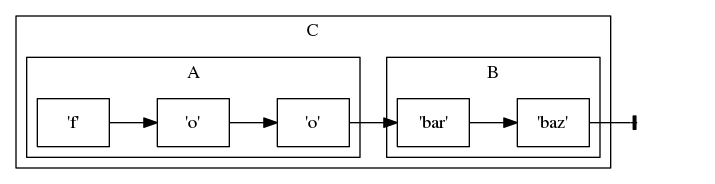
\includegraphics[width=11cm]{./graphs/hblconcat.png}
	\caption[Concatenation of two horizon-based linked lists]{Concatenation of two horizon-based linked lists. The boxes denote the scope, or horizon, of each value.}
	\label{fig:hblconcat}
\end{figure}

This design is enough in our case to cover most uses, because string insertions are not possible in PL/SQL. Therefore, only allowing appending and prepending values is enough. To accelerate typical accesses, we keep the total length of the \varchar{} value in a field.

This design is very similar to the rope representation, but has many benefits in our particular case. First, the structure is flat, i.e. always has one layer, which simplifies iteration over the value. This is a common operation which is required when converting the value back into a buffer before returning. No virtual calls are necessary, and we can read the whole value inside a very simple loop. This flat structures also simplifies the escape analysis, and allows the compiler to virtualize the list in simple cases.

\subsection{Canonicalization}

%\begin{itemize}
%\item easy adding new builtins through canonicalization
%\item can then specialize / optimize those builtins for better performance
%\item not always useful to handle all data types, could be better to ask for canonicalization
%\item can use that as a fallback for simpler implementation
%\end{itemize}

The design presented so far still has a flaw. While it is possible to prepend to a list indefinitely, only one append is possible. In the case a second append operation is required to the same prefix, the latter must be copied, which incurs a high cost. We now present an optimization for this case, which can be used for other purposes.

First, note that the case mentioned is uncommon. Indeed, programs tend to extend the same string all the time, leading to various forms of a "string building" workload. In this scenario, strings are constructed by appending a lot of small elements to the same variable. However, reusing that same prefix for another concatenation is rather uncommon. This is especially true for the short-lived strings we work on.

But this is hardly the only case which requires our system to perform a copy. Substrings on list values must also perform a copy. Recall that the list values we use are immutable. It is therefore not possible to change the indexes in a base value without changing the value of the whole list. Adding substring indiexes is not a solution either, because it does not allow for the simple concatenation method we used so far (think about appending a substring-ed list to another, the indexes would conflict). Therefore, building a substring of such value requires a copy of the entire list, or at least of the complete \varchar{} value.

%Indeed, internal list pointers cannot be changed once assigned a first time, and the values pointed to are immutable as well. This is necessary to ensure the immutability of the overall value.

This becomes problematic if a program follows the pattern shown in \ref{fig:substrcanonpattern}. When multiple substring operations are performed on the same concatenation result, multiple copies of the same value are done. This pattern is more common than the previous one, as using substrings in a loop is the only way to iterate over the characters of a \varchar{} value.

\begin{figure}[tb]
	\begin{subfigure}[h]{\textwidth}
		\begin{lstlisting}[style=PLSQL, frame=L]
prefix := root || dir || subdir;
patha := prefix || filea;
pathb := prefix || fileb;
		\end{lstlisting}
		\caption{Appending multiple times to the same prefix}
	\end{subfigure}
	\,
	\begin{subfigure}[h]{\textwidth}
		\begin{lstlisting}[style=PLSQL, frame=L]
fullstr := a || b || c;
x := SUBSTR(fullstr, 1, 5);
y := SUBSTR(fullstr, 6, 10);
z := SUBSTR(fullstr, 11, 15);
		\end{lstlisting}
		\caption{Multiple substrings on the same concatenation result}
		\label{fig:substrcanonpattern}
	\end{subfigure}
	
	\caption{Example of patterns that require multiple copies of a list value.}
	\label{fig:canonpatterns}
\end{figure}

To solve this problem, we first make a few remarks. Note that these problems are due to the same concatenation result being used in different operations. This can only happen if the concatenation result has been stored and re-read later. In our system, this means the problematic value is necessarily coming from a variable read.

The solution is to use a canonicalized form of the value. Every \varchar{} value in our system can be represented as a base value. This is trivially true for base values, but is also the case for lists as we can flatten them into a heap value. Substring and concatenation on these base values is very fast and always works the same way. To remove the duplicate copies, we add a specific node, when building the AST, that ensures the input to substring nodes is always canonicalized. If the said value is produced by a variable read, the flattened value is written back to the frame. Consecutive substring operations are performed on the already-flattened value, which can be read from the frame with no additional cost. We do a similar optimization for concatenation in the conflicting case.

This is still not perfect. It has some room for further optimizations, and creates other inefficient patterns, but it is a step in the right direction, and makes inefficient patterns even more rare. On top of that, with the assumption that we usually handle short strings, flattening lists could be more efficient than copying the list itself.

\subsection{Null support and empty strings}

%\begin{itemize}
%\item null handling
%	\begin{itemize}
%	\item empty string is null as well
%	\item null is an empty string
%	\item ex: '' = '' is NULL ! (or IS NULL '' is true)
%	\item btw, what happens to length of the empty string ?
%	\item we need specializations for these as well
%	\item choose solution, but most likely separate null and empty string completely and disallow for empty strings to be created
%	\item this way, types for varchar values only contain live non-null strings
%	\item need to benchmark it without necessarily putting it in the report
%	\item means more specializations and checks, but not much more than that
%	\end{itemize}
%\end{itemize}

A major specificity of the \varchar{} type is the handling of empty strings. In PL/SQL, an empty string is \plsnull{}. This can be confusing, especially when statements like '\pls{IS NULL ''}' do not yield false as expected, but true.

Without diving into the details, let us say that this semantics is very simple to get in the database PL/SQL interpreter, due to the value representation. However, we now have multiple kind of values to represent strings in our Truffle interpreter, and each of them should be checked for emptiness whenever performing an operation. This also means that null checks are way more complex : they are not bound to the singleton value we used so far, but can be represented in a variety of ways.

To simplify this, we disallow the creation of empty strings, and replace these by the singleton null value we used so far. Note that only the creation of heap values must be checked this way. Indeed, empty native strings are directly inputted to the program as \plsnull{} values. List values must have at least one element, which is a base value, and we already know that base values cannot be empty, so list values cannot be empty either.

This might make the type analysis harder for Graal, as the return type of some operators is only bound by the supertype \java{Object} (\varchar{} and \plsnull{} values have no common ancestor in the type hierarchy). This can become a problem and degrade performance. Note that guard elimination would have become harder anyway, would we have kept empty strings. Some type guards would have been replaced by field-checking constraints, verifying that the length is greater than 0, and such guards are way harder to optimize for Graal than type guards.

\subsection{Builtin support}

%\begin{itemize}
%\item \varchar{} only used through builtins
%\item need to provide implementation as Truffle node for performance
%\item extensible through canonicalization
%\item replace impl based on substring and concat
%\item also uses canonicalization
%\end{itemize}

Because builtins are the only way to use \varchar{} values, it is very important that we provide support for a good number of core builtin functions. We currently have concatenation (\pls{||}), \pls{SUBSTR}, \pls{REPLACE} and \pls{LENGTH}. These have been chosen because they are among the most commonly used operators, and because they are enough to program a lot of basic functionalities one would want for \varchar{}.

We already talked about the implementations of concatenation and substring. It is interesting to note that the \pls{REPLACE} implementation we have uses concept from both of these. In our system, replacing pieces of a string does not require any copy or buffer transfer. Instead, it is the concatenation of substrings provided as input. Any part of the input string that does not match the given pattern can be reused in the result, and the replacement string can be reused wherever the pattern does match. This means re-using the buffer of the input values, without performing any copies, as shown in example \ref{fig:replaceexample}. Because we want to use the replacement string multiple times in a concatenation, we need to have it as a base value. For that, we use the same canonicalization optimization we used for substrings.

\begin{figure}[h]
	\centering
	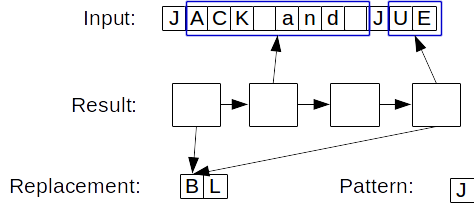
\includegraphics[width=9cm]{./graphs/ReplacementExample.png}
	\caption{Result of the operation \pls{REPLACE('JACK and JUE', 'J', 'BL')}, using list representation}
	\label{fig:replaceexample}
\end{figure}

In addition to the builtins we implemented so far, we also built an extensible framework, which allows for adding new builtins easily. Conversions from the input types to the ones matching the signature of the builtin are made automatically. Finding and creating a node for such operations, using only the name of the builtin is also simple. Finally, using canonicalization can be a very easy way to implement builtins without providing support for all the different representations we can have in the interpreter. Basic support for the base values is the only thing necessary. Of course, supporting list values without requiring them to be flattened is more efficient, but this solution can be used to quickly expand the set of supported builtins with a small amount of work.

\subsection{Shortcomings}

%Because we target a very-specific workload, clearly possible to "ruin" the performance by doing exactly the opposite (give specific examples)

%\begin{itemize}
%\item solution has large memory overhead
%	\begin{itemize}
%	\item give pointers on how to reduce it ?
%	\item largely due to java pointer/reference size
%	\end{itemize}
%\item linked list solution leads to a lot of allocation
%\item can be lowered if values are correctly escaped analyzed (can we check if it is the case ?)
%\item upper bound
%	\begin{itemize}
%	\item possible virtualization helps
%	\item example of replace with replacement bigger than pattern for sharing improving mem consumption (still overhead tho)
%	\end{itemize}
%\end{itemize}

The solution we presented in this section is more performant than a naive buffer-and-copy design. But it does suffer from drawbacks, some of which we already addressed with specific optimizations earlier.

The major drawback of this method is the memory overhead. Indeed, when concatenating, new allocations are made both for the new linked list node and the encapsulating horizon-based list. Each linked list node contains a pointer to its value, plus a pointer to the next node. The HBL contains a pointer to the first node, a pointer to the last node, the number of nodes, and the length of the total string value. The base values contain a pointer to the buffer (be it in the heap or coming from the external C environment) plus a starting index and a length. With 32-bit ints and 64-bits pointers, the overhead for the result of n concatenations is :

\begin{align*}
overhead(n) &\leq sizeof(\java{HBL}) + n \times (sizeof(\java{LinkedListNode}) + sizeof(\java{BaseValue})) \\
			&= (8+8+4+4) + n\left[(8 + 8)+(8+4+4)\right]\\
			&= 24 + 32n \ \text{bytes}
\end{align*}

This is a high cost to pay, but allows us to have very efficient operators implementation. Note that this formula is only an upper bound for the overhead, because measuring the actual memory consumption requires runtime information. This result is based on the assumptions that the sub-results of the concatenation are not shared, and that no base value in that list is shared anywhere else (or appears twice in the list). This last assumption is hard to verify of course, but does not seem reasonable. Making the inverse assumption leads to an overhead of $24 + 16n$ bytes, which is almost half for long lists. Finally, note that the size of the buffers is not taken into account because it does not create overhead (it is necessary for very naive approaches as well).

Even though this method has a high memory overhead, it is possible in certain circumstances that the size of our structure is smaller than the actual string length. This could occur if the string is constructed by always appending the same value. In this case, the base value boxed and buffer is reused everywhere. If the string appended is longer than the size of the linked list node, then memory is saved. As computed, the appended string would need to be longer than $16$ characters long.

Another problem with the current design is the fact that there still is some polymorphism in the values. Indeed, linked list nodes could either point to native or heap values. Although length and starting index fields can be factored out and granted access to without knowing the actual type, accessing the value itself (the buffer) requires a type check at runtime. This removes optimization opportunities for Graal, and makes virtualization much harder. Lack of virtualization in this case can be really damaging for performance, as it would require a lot of allocations at runtime, and incur great stress for the garbage collector. We describe some ways to alleviate this problem in section \ref{sec:futurework}.

%\cleardoublepage
\startsection{Performance evaluation}
\label{sec:benchmarks}

In this section, we show the performance of our system when compared to the database execution engines. We then validate the different design decisions taken. We close by looking at the memory consumption of the system.

%What do you want to show ?
%\begin{itemize}
%\item faster than the DB
%\item null-handling better this way : re-implement one or two operators and check
%\item string design better than classic/naive copy from DB then all in JHeap
%\item string design better than copy only when necessary
%\item show memory consumption ! possibly better than the DB (interesting since VARCHAR2 usage typically declares max size or 1000 characters)
%\item recognizing patterns and implementing them in particular is both easy and has a big impact
%\item how impactful single operation implementation + representation(s) used are
%\end{itemize}

\subsection{Database integration}

%How we did it (briefly) :
%\begin{itemize}
%\item stub compilation then loading, parsing, building and execution
%\end{itemize}

In order to perform a fair comparison of the database and our Truffle interpreter's performance, we must run the same programs, and in the same context. Because normal PL/SQL can't be run outside of the database, we must find a way to integrate our interpreter into the database. This will allow to run typical PL/SQL workloads, as part of SQL queries on big tables, and lead to a working prototype for this project.

We want to be able to perform SQL queries with PL/SQL code in it. The only thing we will be concerned about is making UDF calls from SQL to PL/SQL work. We already discussed some form of database integration in the extraction of the DIANA code. We will use the same system parameters to guide the interception of SQL calls to PL/SQL.

First, we must store the JSon representation of the DIANA tree into the database. Using the same code as when we extracted the DIANA to an external file, we adapt it to store the resulting JSon in the database space pre-allocated for the function metadata.

Intercepting PL/SQL UDFs in SQL queries is done the same way as the dbjs project does it. When the SQL query is compiled, we identify all the PL/SQL calls it makes. For each of those, we verify if we already produced JSon for it. In this case, we replace the call by a Truffle stub generated on the fly. This stub is responsible for understanding the database's function call convention, and performing the required conversions before executing the Truffle AST for this function with the correct arguments.

Although we do support native database values, we still need to perform conversions for values of type \oranum{}. Our Truffle interpreter does not provide support for the latter, but has to accept them. This is due to SQL's type system, which does not contain integer types. The stub is then useful for checking that the numbers passed are indeed integer values, and then converting the database value into a Java integer. Once our AST interpreter returns the final result, the stub is also responsible for converting it into a value understood by the database. This might mean converting Java \java{int} back into \oranum{}, or copying any internal string value representation into a C buffer.

To be able to run our interpreter inside the database, we build an SVM image, and link it to the database. Calls from the database code to the Java portion is handled by SVM.

\subsection{Methodology}

%\begin{itemize}
%\item micro benchmarking only
%\end{itemize}

We now measure the performance of our system using different metrics. We will showcase the improvement it provides when compared to the current database options, and use these results to validate our design decisions. For the latter, we will specifically measure the cost of null handling, as well as the performance of simpler string implementations.

To get significant results that mimics the typical use of PL/SQL, we try to devise benchmarks that follow the basic workloads of this language. We will focus on two abstract concepts, both used as part of an SQL query. The first workload considered is User-Defined Functions (UDFs), which are very short functions, performing only a few operations. The second will be closer to Stored Procedures use (STP), with longer-running program, using loops. We measure performance only using micro-benchmarks, written for this project.

We run these programs as part of SQL queries, either in the \sql{SELECT} part or in the \sql{WHERE} clause. Site of use does not impact performance at all. We run these queries on randomly-generated tables of 10 million entries. We measure the running time of the query itself, and average the results over 5 runs.

We compare the performance of the Truffle interpreter we implemented for this project (noted as \truffle{}) with the different systems that already exist in the database. The two traditional modes of execution are measured, i.e. the PL/SQL interpreter (\pvm{} for PL/SQL Virtual Machine), and the native compilation option (\ncomp{}). To get the best performance out of these, and also to measure the ratio between PL/SQL execution and database-to-PL/SQL context switching time, we use the \pls{PRAGMA UDF} option that PL/SQL provides. This annotation can be added in the code, and tells the compiler that this function will primarily be used in the context of an SQL query. Special care is then taken by SQL when calling this function, to get rid of some of the context switching cost. For this optimization to be possible, some restrictions on the programs are necessary, and are explained further in the documentation. These improved systems are noted \pvmg{} and \ncpg{}.

\subsection{Numeric benchmarking}

%\begin{itemize}
%\item only \simpleint{}
%\item we recall that not null and classic overflow
%\item should be most efficient numeric type
%\item simple mem representation
%\item super CPU friendly
%\item must be converted because no support for \oranum{} and database only knows this
%\item give example of program that has conversion in it (with signature)
%\item give speedup compared to \ncpg{}
%\item separate the benchmarks (single op, exp, special)
%\item quick note on const and search
%\item most cost in conversion
%\item we have a stub that is already specialized
%\item need more thorough stuff to get perf of PL/SQL itself
%\item programs very short so PL/SQL code not the only story here
%\item simple to see that computation not interesting because ncomp not better (same perf)
%\end{itemize}

\subsubsection{UDF case}

We first show the performance of the different systems on very simple, UDF-like numeric benchmarks.

We show in this section the execution speed of \simpleint{} programs. We recall that this type is the simplest numeric type that PL/SQL provides. It cannot be \plsnull{}, is represented by a 32-bit integer in memory, and has no specific overflow semantics. This is the most CPU-friendly type, and should therefore be the most efficient.

However, the only numeric type the database understands and supports is \oranum{}. Therefore, to be able to run programs using a different type, we must first perform a conversion operation. Every program in the set of benchmarks used will have such a conversion as its first operation. Such a conversion will also be necessary when returning the value. We show an example in Figure \ref{fig:mulbench}.

\begin{figure}[hbt]
	\begin{lstlisting}[style=PLSQL, frame=L]
FUNCTION mul(a NUMBER, b NUMBER) RETURN NUMBER IS
	c SIMPLE_INTEGER := a;
	d SIMPLE_INTEGER := b;
BEGIN
	RETURN a * b;
END;
	\end{lstlisting}
	\caption{Code for the \bench{mul} benchmark}
	\label{fig:mulbench}
\end{figure}

The results for all the benchmarks are shown in Figure \ref{fig:exp1a}. The programs ran are all very short to mimic a UDF workload. The first three use only a single operator, the following four show more complex mathematical expressions. Then, \bench{const} performs an empty call that only returns a constant, to show the cost of context switching, and \bench{search} implements a very simple compare-and-return function that showcases the performance of comparisons and control flow operators. For each system, we measure its performance as the speedup it achieves compared to the \pvm{} baseline.

\begin{figure}[tp]
	\centering
	\makebox[\textwidth][c]{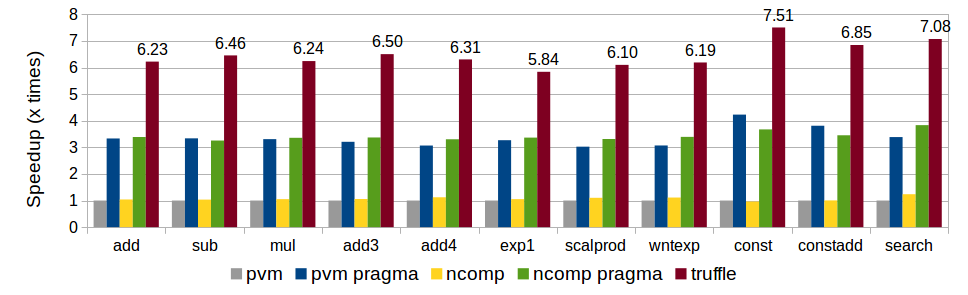
\includegraphics[width=16cm]{./results/exp1a.png}}
	\caption[Execution speed of the \simpleint{} UDF benchmarks]{Execution speed of the \simpleint{} UDF benchmarks (lower is better)}
	\label{fig:exp1a}
\end{figure}

We can clearly see that the major costs for the basic systems is given by the context switching, because using the \pls{PRAGMA UDF} annotation improves performance by almost 3.5 for every benchmark. The \truffle{} interpreter is even better, and divides the execution time of the \benchsystem{pragma} systems by nearly two (1.84x on average).

The performance gain comes mostly from the stub implementation. Indeed, this layer of interaction between the database and the Truffle PL/SQL interpreter performs the conversion from the complex representation of \oranum{}s to Java-based ones, does the checks for input \plsnull{} values, and is also written as a Truffle AST. It therefore benefits from specialization, and can make assumptions, for example that the input value is never null, because none was ever found. We also reused existing blocks that implement an efficient conversion from \oranum{} to integers, using specialization. Finally, the input programs are so short that very few time is actually spent executing the code, most of it is dedicated to conversions and interfacing with the database.

These numbers are very good, but do not tell the whole story. They measure the efficiency of a highly-specialized module we did not write, and gives very few insight into the performance of the different PL/SQL execution engines. To solve this issue, we now focus on more computation-intensive benchmarks, with longer running times, to show the speed of the PL/SQL execution, while still in a believable workload.

\subsubsection{Stored procedures}

Stored procedures are typically more computation-intensive than UDFs as they may use loops and temporary variables. These could be used to filter some results according to a complex criteria. An example could be the following query : \sql{SELECT * FROM datapoints WHERE gcd(a,b) = 1}.

\begin{figure}[tp]
	\centering
	\makebox[\textwidth][c]{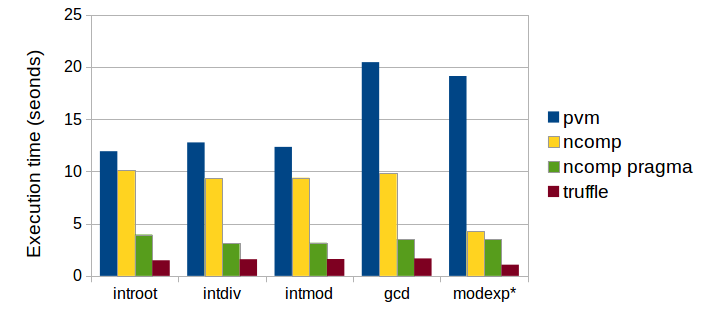
\includegraphics[width=13cm]{./results/exp1b.png}}
	\caption[Execution speed of the stored procedures benchmarks]{Execution speed of the stored procedures benchmarks\\
			\hspace*{-5cm}*\textit{scaled down}}
	\label{fig:exp1b}
\end{figure}

We devise a second set of benchmarks, comprised mostly of loop-based functions, with a varying degree of computation involved. Once again, these only use the type \simpleint{}. Results are shown in Figure \ref{fig:exp1b}. The benchmarks are sorted from the least computation-intensive to the most computation-intensive.

We can already see that the time spent executing the PL/SQL code is longer, because the use of \pls{PRAGMA UDF} onlt gives a speedup of 2.5 for the first benchmark, and does not give any improvement for the heavy \bench{modexp} benchmark. This observation is reinforced by the improvement given by the \ncomp{} system. Though not providig any speedup in the UDF case, it is now showing an improvement between 1.20x and 4.50x  over the \pvm{}. The speedup provided by our Truffle interpreter also increases. Between 6x and 7x for the previous set of benchmarks, it is now between 8x and 18x for the most computation intensive functions. This is a good sign that the PL/SQL implementation we provide has better performance than the builtin systems. If we compare the improvement over the \ncpg{} variant, which is the most efficient of the classic options, we get a speedup between 1.95x and 3.25x, averaging at 2.40x. These are very good measurements, and showcase a real improvement over the database implementation of PL/SQL.

\subsubsection{Computation intensive benchmarks}

To complete this numeric experimentation, we try to get rid completely of the conversion and context switching cost. To do that, we implement two very computation-intensive functions in PL/SQL, that will be called only once on a single-entry table. Although not interesting in itself because it does not show performance for a typical use of PL/SQL, this experiment will be useful in determining the actual speedup that comes from executing PL/SQL code with our alternative.

%\begin{figure}[tp]
%	\centering
%	\makebox[\textwidth][c]{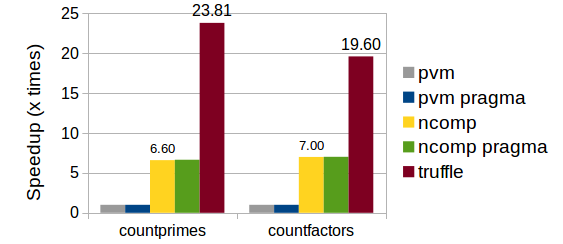
\includegraphics[width=12cm]{./results/exp1c.png}}
%	\caption{Speedup for computation-intensive \simpleint{} benchmarks. Speedup is measured compared to \pvm{} (higher is better).}
%	\label{fig:exp1c}
%\end{figure}

The two functions implemented and measured respectively count the number of primes from 1 to 50'000, and count the number of prime factors every number from 1 to 20'000 has. Figure \ref{fig:exp1c} shows the results. We can see that the overhead of context-switching has been removed completely, as using \pls{PRAGMA UDF} does not give any improvement anymore. The native compilation option also provides its maximal speedup, as advertised in the Oracle documentation, of 7 times the performance of the PL/SQL intepreter (\pvm{}).

The Truffle interpreter we implemented goes way further, and reaches up to 24 times the performance of the \pvm{}. This is mostly due to Just-In-Time compilation technology, that uses all the runtime information available to produce very efficient code. Branches and input values can be profiled, and complex three-valued logic based conditions can be reduced to the normal boolean case because no \plsnull{} condition is ever encountered. More generally, no \plsnull{} checks must ever be performed in any operator, because it is known that this program only handles \simpleint{}. Though we did not encode this specifically when parsing the program, Graal found out itself by profiling the seen values. The native compilation option provided by the database cannot do such a task, and uses more general comparison and branching operators that must perform the checks, even though they are unnecessary. Finally, the \ncomp{} system does not reach the optimal performance of a hand-crafted C program that would do the same task as implemented in PL/SQL, because it is performs heavy calls in a shared library to perform most of its operations. These calls are not easily optimized by classic C compilers (e.g. gcc), and thus do not give the CPU-instruction execution speed we could expect. The speedup of our Truffle interpreter when compared to the \ncomp{} option is 3.60x for the \bench{countprimes} benchmark, and 2.80x for the \bench{countfactors} benchmark. The speedup achieved is still dependent on the function, but is a very impressive result, keeping in mind the simple AST interpreter we wrote in Java.

\begin{figure}[tb]
	\centering
	\vspace{4mm}
	\begin{subfigure}[c]{0.4\textwidth}
		\centering
		\caption{Execution speed (seconds)}
		\begin{tabular}{|l|r|r|}
\cline{2-3}
\multicolumn{1}{c|}{} & countprimes & countfactors \\
%			& countprimes & countfactors \\
\hline
pvm 			& 37.14 & 37.50 \\
ncomp		& 5.63 & 4.93 \\
ncomp pragma & 5.59 & 4.92 \\
truffle		& 1.56 & 1.76 \\
\hline
		\end{tabular}
	\end{subfigure}\hspace{3cm}%
	\begin{subfigure}[c]{0.4\textwidth}
		\centering
		\caption{Speedup achieved}
		\begin{tabular}{|l|l|r r|}
\cline{3-4}
\multicolumn{2}{c|}{} & pvm & ncomp \\% \hline&			& pvm & ncomp \\
\hline
count	& ncomp		& 6.6 & - \\
primes	& truffle	& 23.8 & 3.6 \\
\hline
count	& ncomp		& 7.0 & - \\
factors	& truffle	& 19.6 & 2.8 \\
\hline
		\end{tabular}
	\end{subfigure}
	
	\caption{Results of the computation-intensive \simpleint{} benchmarks}
	\label{fig:exp1c}
\end{figure}


\subsection{Impact of \plsnull{} handling}

\subsubsection{Changing the type}

To continue our performance evaluation, we now turn to the second integer type we implemented. This will be interesting to see the added cost of null checks and specific semantics in the case of overflows.

The first experiment we run is very simple : we take the exact same benchmarks we ran earlier, and switch the types. Instead of using \simpleint{}, every input is converted to \plsi{} instead. At first glance, that does not seem to change anything, but it does have some impact.

First, because \plsi{} accepts the \plsnull{} value, execution now has to take this possibility into account. This is done through null checks in the basic operators, and should increase the running time. The second reason is the overflow semantics of the \plsi{} type. Indeed, values of this type are guaranteed not to overflow. Therefore, every arithmetic operation performed on it must ensure that no overflow occurred. This is slowing down every single operation, and increases the running substantially.

\begin{figure}[tp]
	\centering
	\makebox[\textwidth][c]{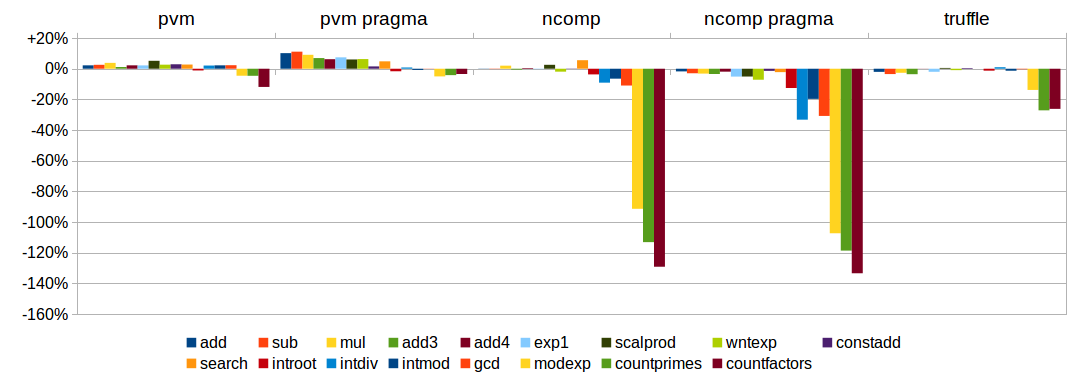
\includegraphics[width=16cm]{./results/exp2a.png}}
	\caption[Impact on performance of using \plsi{} instead of \simpleint{}]{Impact on performance of using \plsi{} instead of \simpleint{}.\\
			\small{}Execution speeds are compared for the same systems, with the two versions of the programs. Positive values show improvement, and negative values show a degradation of performance.}
	\label{fig:exp2a}
\end{figure}

We run these modified benchmarks, and show the results in Figure \ref{fig:exp2a}. For each benchmark, we measure the execution speed degradation of every system, compared to the same system on the \simpleint{} version of the function. This shows the impact on every evaluated system of changing the used type, without actually encoutering the \plsnull{} value, because we run the queries on the same tables (that do not contain any \plsnull{} value). All the benchmrks are shown sequentially, from the least to the most computation-intensive.

First, notice that the \pvm{} behaves unexpectedly. For most benchmarks, i.e. for the UDFs and stored procedures, using \plsi{} acutally improves performance. This is amplified when using \pvmg{}, as the latter is more sensitive to changes in PL/SQL execution time, and reaches 10\% on some benchmarks. The reason for this is the fact that conversion is now slightly simpler, as \plsi{} does accept the \plsnull{} values, if one was encoutered in the table. Because the UDF programs are very short, this lighter conversion cost compensates for the more expensive \plsi{} operator. This ratio is inverted when running more computation heavy benchmarks, leading to up to 12\% degradation for the last function.

The native compilation behaves very differently. We can see that changes in the execution time is very small in the case of UDFs (between +5\% and -5\%). This slowdown remains reasonable for stored procedures (10\% slowdown for \ncomp{}), but already becomes significant on these same functions when using the \pls{PRAGMA UDF}, for the same reason as above : a 30\% slowdown is a heavy cost for just changing the data type used. But the huge slowdown comes from the most computation-intensive benchmarks. The program's execution takes twice as much time to complete when compared to the \simpleint{} case. This cost is due to the more expensive operations that \plsi{} supports. Indeed, the very good performance of this system on the heavy benchmarks was due to CPU-friendly operations, that could be performed natively. In that case, some of the operators could be transformed directly into a single CPU instruction. However, with the more complex \plsi{} semantics, every operation now needs to check if some of the operands are \plsnull{}, and if the operation execution did overflow. This is a heavy cost to add to every operation, which now performs conditional-branching even for the simplest arithmetic expression.

The Truffle interpreter does not have that problem. As we can see, there is some slowdown on almost every program, but it is very small for the simplest programs (less than 3\% for the UDF and stored procedures). For computation-intensive benchmarks, the maximum slowdown observed is 27\%. This is still a big price to pay for only changing the data type, but is much smaller than the native compilation, which showed the best performances on these programs. In fact, the operators are still more expensive in the Truffle AST, because overflow checks cannot easily be avoided (this would require profiling on every operand of every operator). However, most \plsnull{} checks can be removed, except the input ones. Indeed, no such value is ever encoutered, meaning that the only data representation flowing during execution of the program is the primitive \java{int} type. This cannot be a null value, and Graal can then make assumptions that this is the only case of interest. This removes all internal checks, which gives a smoother degradation. The initial checks must still be performed on the input values, because no information about these external values coming from the database is known. With this smoother degradation, we reach up to 6x speedup over the best database implementation (\ncpg{}), with an average of 2.75x.


\subsubsection{Multi-specialized nodes}

We now discuss the encounter of the \plsnull{} value, and its effects on the Truffle interpreter. This is especially interesting because it showcases the added cost of having multiple specializations active at the same time in some nodes. This requires the node to take the decision on which implementation to use at run-time, and reduces the opportunity for speculative assumptions. Because this is a Truffle-specific problem, we only measure our interpreter for this experiment.

Measuring the impact of the \plsnull{} value on performance can be tricky for PL/SQL programs. Indeed, this is a special case that is thought to be quite uncommon, but still has a complete set of semantics attached to it. Comparisons with \plsnull{} yield \plsnull{}, and branching on \plsnull{} takes the false branch. Loops are thus avoided if based on a \plsnull{} comparisons, and directly go to the end. This means that for our loop-based programs (stored procedures and more computation heavy programs), the main body of the program is usually not executed at all. Measuring the change in execution speed for various amounts of \plsnull{} is then not very useful.

Instead, we will apply the benchmark queries we used so far on similar, but not exactly identical tables. The baseline will be measured on the same tables we before, with no \plsnull{}. We then measure the first variant on the same table, with one \plsnull{} entry added. This entry has one null field, and all the others remain classic values. The second variant has one added entry per column, with each such entry having exactly one \plsnull{} field. An example is shown in Figure \ref{fig:nullvartabs}. Once the programs have been run on these alternative tables, the Truffle nodes have more than one specialization active at the same time. Re-running the program on the same table allows us to measure the time taken by the generic code. This gives us the degradation when the code is not perfectly specialized, and has to take care of all the possible inputs.

\begin{figure}[h]
	\centering
	\vspace{6mm}
	\begin{subfigure}[t]{0.3\textwidth}
		\centering
		\caption{Basic table}
		\begin{tabular}{|R|R|R|}
			\hline
			a & b & c \\
			\hline
			1 & 2 & 3 \\
			-1 & 0 & 17 \\
			501 & 7 & 1042 \\
			\hline
		\end{tabular}
	\end{subfigure}
	\begin{subfigure}[t]{0.3\textwidth}
		\centering
		\caption{One-null variant}
		\begin{tabular}{|R|R|R|}
			\hline
			a & b & c \\
			\hline
			1 & 2 & 3 \\
			-1 & 0 & 17 \\
			501 & 7 & 1042 \\
			\plsnull{} & 2 & 1 \\
			\hline
		\end{tabular}
	\end{subfigure}
	\begin{subfigure}[t]{0.3\textwidth}
		\centering
		\caption{All-null variant}
		\begin{tabular}{|R|R|R|}
			\hline
			a & b & c \\
			\hline
			1 & 2 & 3 \\
			-1 & 0 & 17 \\
			501 & 7 & 1042 \\
			\plsnull{} & 2 & 1 \\
			13 & \plsnull{} & -100 \\
			1 & 503 & \plsnull{} \\
			\hline
		\end{tabular}
	\end{subfigure}
	
	\caption{Example of the \plsnull{} variants of the tables used for the multi-specialization experiment.}
	\label{fig:nullvartabs}
\end{figure}

The results of this experiment are shown in Figure \ref{fig:exp2b}. We can see a small increase in the '1 NULL' case for every benchmark. The 'all-NULL' case is always the slowest case of all. This makes a lot of sense because it means more nodes have actually been affected by the \plsnull{} values. The middle case is interesting because it shows that a single \plsnull{} value, though altering the performances, only leads to a small increase (less than proportional) in execution time. This is due to the fact that only a few nodes have been affected. When all the columns are null one after the other, way more nodes are affected, leading to poorer performances. This change is greater when the program is computation-intensive, as in the case of \bench{modexp}, as the checks added by multi-specialization must be performed many times. This leads to the biggest degradation of all, peaking at +50\% running time.

\begin{figure}[tp]
	\centering
	\makebox[\textwidth][c]{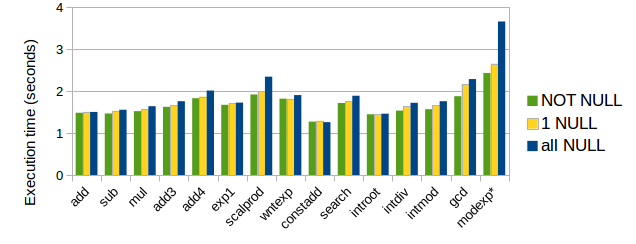
\includegraphics[scale=1]{./results/exp2b.png}}
	\caption[Execution time of the Truffle interpreter in the multi-specialized case]{Execution time of the Truffle interpreter in the multi-specialized case.\\ 			\hspace*{2cm}*\textit{scaled down}}
	\label{fig:exp2b}
\end{figure}

Combining this increase in running time plus the degradation due to the type change from \simpleint{} to \plsi{}, we get a total slowdown of 1.9, which is still smaller than the 2.2 slowdown of the native compilation when changing the used type. This is due to the fact that not all nodes of the AST are affected by this change. For example, the code that is in an if-branch, or in the body of a loop, is never executed with the value \plsnull{} because the condition evaluates to false. This means that the condition has multiple specializations and is slower, but once in the body of the loop, only integer values are known to appear. This kind of optimizations and very localized specialization is only possible using runtime specializations, and allow the code to be generic only where it needs to be.


\subsection{\varchar{} performance}

\subsubsection{Comparison with the database}

%\begin{itemize}
%\item explain input and output copies
%\item no conversion like in the integer case
%\item small programs (one line) means small room for improvement
%\item explain the benchmarks !
%\item builtin calls also slightly more efficient !
%\item show lists are correctly virtualized / escape analyzed in simple cases
%\end{itemize}

We now evaluate the performance of our \varchar{} implementation. The methodology is very similar to the numeric case. We perform micro-benchmarking on SQL queries ran on tables of 10 million entries. The difference will come from the systems compared. When running \varchar{}-based programs, the difference between the interpreter and the native compilation is rather small. This is due to the nature of string operations on immutable values : they tend to involve a lot of copies. Furthermore, the result must be stored in a specific buffer. Therefore, a copy is always necessary, if only just to return the value.

We start once again with the UDF case. We wrote a set of very small, UDF-like programs, calling the \varchar{} builtins we implemented. Results for these benchmarks is shown in Figure \ref{fig:exp3a}. We can see a steady improvement over almost all the benchmarks. In some cases, the speed of our interpreter is the same as what could be achieved before, but it is never worse. Overall, we get a 25\% improvement in execution speed.

\begin{figure}[tp]
	\centering
	\makebox[\textwidth][c]{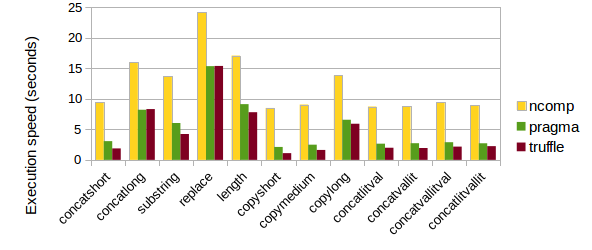
\includegraphics[scale=1]{./results/exp3a.png}}
	\caption{Execution speed for the \varchar{} UDF benchmarks}
	\label{fig:exp3a}
\end{figure}

This result is not as good as the speedup we achieved in the \simpleint{} case for UDFs. The main reason for that is the lack of conversion. In the numeric benchmarks, every input value had to be converted. This operation was done using code specialization, which is more efficient than doing it normally. Furthermore, due to the need for a copy of the result into the output buffer, a significant portion of the execution time is dedicated to unavoidable buffer copy, and that for every evaluated system. The cost of such a copy is made explicit in the \bench{copyshort}, \bench{copymedium} and \bench{copylong} benchmarks.

Another interesting thing to note here is the fact that the cheaper context switching Walnut provides us allows us to outperform the database. Otherwise, these benchmarks are too simple to give any room for optimization. For example, in the \bench{concatshort} case, the operation must take the two input buffers, and copy them both into the output buffer. There is no way around it, and not really anyway to speed that process up. However, we still get a 55\% improvement on this benchmark, due to the optimized context switching. Notice that this does not translate to more intensive benchmarks, like \bench{concatlong}, because the longer time spent copying the buffers minimizes the impact of context switching. On such benchmarks (\bench{concatlong} and \bench{replace}), we get no improvement with our solution, but we do not perform worse. This shows that the solution we use reaches the speed of the most simple and bare-metal solution for basic operations.

To get some benefits from our complex solution, we must increase the amount of computation performed. As we did before, we devise another set of benchmarks, more computation-intensive, which we'll say represent a stored procedure workload. We run these programs on the same number of table entries (10 million). We present these results in Figure \ref{fig:exp3b}.

\begin{figure}[tp]
	\centering
	\makebox[\textwidth][c]{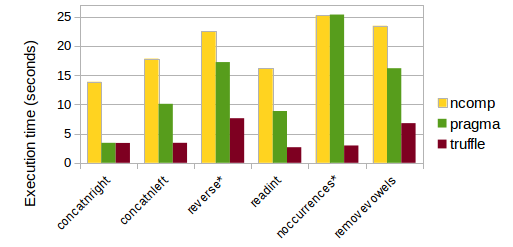
\includegraphics[scale=1]{./results/exp3b.png}}
	\caption[Execution speed of the \varchar{} stored procedures]{Execution speed of the \varchar{} stored procedures\\
			\hspace*{-4cm}*\textit{scaled down}}
	\label{fig:exp3b}
\end{figure}

The first thing to note here is the difference in behaviours between the \bench{concatnright} and \bench{concatnleft}. These two programs build a string by appending (resp. prepending) $n$ times the same string, where $n$ is an input. In the database systems (both \ncomp{} and \ncpg{}), building a string by prepending takes a lot more time then when appending, although the arguments to the functions are the same. This is typical of classic concatenation algorithms, where one would over-allocate the buffer, and keep appending to the current value, like the \java{StringBuilder} class in Java. Although this method is very efficient when building strings by appending, prepending becomes very expensive because a new buffer must be allocated every time, and the current value must be copied. Our solution does not suffer from this, because appending and prepeding are done without copy, by updating a data structure.

Another interesting thing to note on these results is the case of \bench{removevowels}. This benchmark performs multiple calls to the \pls{REPLACE} builtin. Although our implementation of this functionality showed no improvement over the \ncpg{} system in the case of a single call, it yields a 2.4x improvement in this benchmark. The reason for it is that \bench{removevowels}, as its name suggests, removes some letters, i.e. it calls \pls{REPLACE} with a \plsnull{} replacement. We took the opportunity to optimize specifically this case. One specialized version of our algorithm thus only deals with deletion cases. This makes the algorithm much simpler, and leads to this significant speedup.

Overall, we get greater improvements in the stored procedure case than when dealing with UDFs. The average speedup over the best database system (\ncpg{}) is 2.7x, with a maximum at 8.5x. This maximum is achieved for the \bench{noccurrences} benchmark, which performs a lot of substrings and comparisons. In our system, the former is almost a no-op (it only adds an index to a runtime value), which explains this huge improvement.

\subsubsection{Impact of having multiple representations}

We just saw that the implementation of \varchar{} we provide is rather efficient, as it never performs worse than the database, and usually has significant speedups. We are now interested in knowing what is the reason for this improvement. More specificaly, we wish to validate our design, i.e. show that the faster execution indeed comes from having multiple data representations for string values, with a specialized representation for fast concatenation.

In order to do so, we re-implement efficiently our system with less data representations available. We will compare the following cases:

\textbf{Only heap values available} (1 representation). This requires copy of input values into Java arrays, allocated on the heap. Although this obviously degrades performance, this variant is the simplest. The fact that only one representation is possible simplifies the implementation, and allows for more specific optimizations that would be cumbersome to write otherwise. We use here classic over-allocated buffers for concatenation, making for cheaper append.

\textbf{Only base values available}. This includes heap values and native values (so 2 representations). The burden of input copy is removed, but implementation has more cases and different specializations. Upon concatenation, values are copied into a buffer, which delays the copy of external values.

\textbf{Full system} (3 representations). This is the system described in this project, containing the first two cases plus the linked-list based representation for concatenation.

To compare these different systems, we run them on the same benchmarks as above. To show the relation between these systems, but also with the database implementation, we normalize the results to the time taken by \ncpg{}. This ensures that the results from the different, high-varying execution time programs can all be shown in a meaningful way. On top of that, it gives us a simple way to see which implementations perform better or worse than \ncpg{}. We display these results in Figure \ref{fig:exp3c}.

\begin{figure}[tp]
	\centering
	\makebox[\textwidth][c]{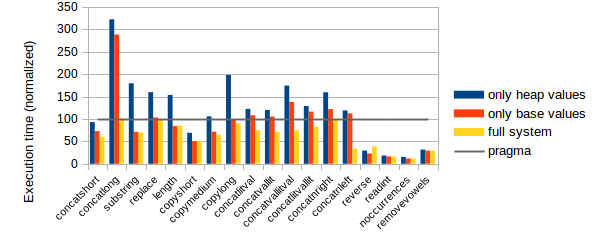
\includegraphics[scale=1]{./results/exp3c.png}}
	\caption[Comparison of the different \varchar{} implementations]{Comparison of the different \varchar{} implementations (lower is better). Execution time is normalized to the time taken by the \ncpg{} system (shown as the horizontal line).}
	\label{fig:exp3c}
\end{figure}

As expected, the first two systems have some additional overhead compared to our full system. This is mainly due to duplicate copy operations. Even in the simplest case, like \bench{concatshort}, both the 1- and 2-representations variants must copy the values to be concatenated into a heap buffer, before copying this value out to the return buffer. Although this very simple case seems easy to optimize, it is very hard to make it work in the general case. This would require us to know where the return value comes from, which cannot necessarily be found statically. This becomes a huge cost when copying large strings, leading to poor performances on \bench{concatlong}. The overhead of the naive approach, i.e. with only heap values, is about +80\% on average when compared to the linked-list solution. This is more than enough to make this system worse than the currently-existing solution (i.e. \ncpg{}).

The second system also performs worse than our complete design. It does remove a lot of useless copies, for example when performing a \pls{LENGTH} or \pls{SUBSTRING} operation. The fact that input values are not always copied is way more efficient. This allows the second variant to approach the performance of the full system. In some cases, they exhibit comparable speeds : \bench{susbtring}, \bench{replace}, \bench{length} ... This is due to the fact that these benchmarks do not use concatenation, which is the main difference between the 2-representation implementation and the final one. For other operators, the specialization path taken by the two versions is the same, because the inputs are always of the same kind (native values). Still, this system is slower than the linked-list approach when it comes to concatenation, because it performs an extra copy into the heap. With this, the overhead averages 37\%. In cases where the complete design was already on par with \ncpg{}, this is enough to tip the balance and make the 'base values only' version slower.

reverse only bench where full system worse : why, how much, how solveable
One can notice that the overheads in the last 3 programs is very small. In the case of the 1-representation case, this is only due to input copy. But the \bench{reverse} benchmark is the only one that goes the other way around : removing data representations actually improved performance ! This speedup is quite significant : 24 \% when using only heap values, and up to 41 \% with support for native values. This benchmark makes heavy use of substring and concatenation operators to reverse the input string. Our design being optimized for concatenation, this should not happen. The reason for this is the fact that the function concatenates a lot of single characters strings in a loop. As we saw when discussing the limitations of our solution, the memory overhead for small strings is significant. Thus, most of the time is spent allocating a lot of memory for wrapping a single character. Because these allocations are performed in a loop, they cannot be escape analyzed by Graal, and the memory must be used. In the simpler variants. concatenating one character is very fast, because it only means copying one character. To solve this problem, we could integrate this buffer-based concatenation for this specific case. By profiling the length of the strings being concatenated, it should be possible to detect this bad case, and use buffers instead of lists. This is left for future work.

overall, our system is the best (ofc) cases where same as db perf, other systems fuck up $\rightarrow$ our complex repr is needed to perform well. even though abstracted, gives best perf, at least as good as native como (not bad !)
Overall, we saw our final solution is performing better than the others. This validates our design, showing that it is possible to improve performances using multiple data representations. When no improvement is possible, our system behaves like the current database implementation of \varchar{}, and never worse. Even though it uses a lot of high-level abstractions, which could represent an overhead in simple programs, these are optimized away by the compiler when possible, and leaves us with the simplest implementation possible. On more complex programs, these abstractions showed their benefits when building strings, copying characters only when the result is complete.


%\subsection{Results}
%
%Note: We won't showcase the degradation due to the database integration, this is only interesting for the PL/SQL team.
%
%\subsubsection{}
%\begin{itemize}
%\item[Goal] Show performance when running inside the database, and how much faster on typical data processing programs and situations (super short programs)
%\item[Benchmarks] In-database \texttt{select} statements with short (believable) programs
%\end{itemize}
%
%\subsubsection{}
%\begin{itemize}
%\item[Goal] Show impact of NULL-handling with specialized null value
%\item[Benchmarks] Compare programs using naive boxing + null value on 0\%, 1\% and 100\% null values in the table column. Do that for both ints and strings.%\newline \textbf{To do very early in the report not to be surprised !}
%\end{itemize}
%
%\subsubsection{}
%\begin{itemize}
%\item[Goal] Show impact of having multiple representations for the VARCHAR2 values
%\item[Benchmarks] Run (previously used ?) short benchmarks, using three VARCHAR2 implementations : 
%\begin{enumerate}
%\item Only heap values
%\item + external value
%\item + concatenation lists
%\item maybe: + an additional tailored representation for one specific operation (kind of already done for concatenation, but do it for another one)
%\end{enumerate}
%\end{itemize}
%
%\subsubsection{}
%\begin{itemize}
%\item[Goal] Show memory usage of the Truffle interpreter, and compare with the database memory usage. This should only consider the resources reserved for the program itself, not the environment.
%\item[Benchmarks] Run some that could really show terrible memory performance for both interpreters, but mostly focus on the previously run (short) benchmarks
%\end{itemize}

%\cleardoublepage
\startsection{Future work}
\label{sec:futurework}

%\begin{itemize}
%\item possibly add more string representations. Could make this less painful by declaring which string rep is accepted for every parameter of the function, and automatically adding wrappers
%\item lower memory footprint
%\item parse diana directly instead of turning into json
%\end{itemize}

Much work can still be done on this project, and this should be a continued effort. We present here some of these future directions, interesting ideas of continued topics, and pointers to solutions that could fix the issues the design chosen still has.

First, for this project to be a complete and correct subset of PL/SQL, a lot of items must be added or fixed. The question still remains open how to prove that our interpreter has exactly the same semantics as the classic execution options for PL/SQL. Answering this question would help acceptation of this solution by potential users. The way it is currently done is through a set of ever-extending unit tests, but this is clearly not enough. More complete testing on full tables queried using SQL could provide more evidence of similar semantics.

Another correctness issue not dealt with is that of concurrency. While we did not provide a mechanism for in-database function call resolution (i.e. a PL/SQL function calling another), adding such a basic feature would require complex and expensive concurrency checks to ensure that the function called still hasn't been modified while the program is running. Although semantics for handling such a case are rather simple in PL/SQL (execution should be aborted by raising an exception), these kind of checks, performed on every call, could prove devastating for the performance of our interpreter.

We showed that language interoperability in the context of Truffle is simple, with the example of \maybe{} the Truffle SQL expression engine. It could be very interesting to try such cooperation with the other languages being added into the database, and ran on the GraalVM. A prime example is JavaScript, which is the most advanced project in this direction. Legacy code written in PL/SQL could then be kept, and called directly from new JavaScript programs running in the database, ensuring the same behaviour can be reproduced.

To improve performance further, there is also a lot to do. For example, a full \oranum{} implementation could be very efficient. Programmers usually tend to avoid this SQL type in computation intensive setups, because of the high cost of operations handling this type. This is all due to the complex memory representation of these, optimized for storage and precision. Using runtime data representation specialization, we should be able to lift this restriction, and use simpler representation when possible. Such work has already been done for the Truffle SQL interpreter, and it would be interesting to integrate this work in a procedural language, with more intensive computations.

To improve on what we implemented so far, we could be using more of the specialized tools Truffle provides. Very small usage of profiling has been done so far, which could improve the performance by simplifying assumptions made by the compiler. Moreover, we did not really touch in that project the subject of implementation-specialization \textit{per se}. We did use type specialization, but it could be interesting to look into very specific code patterns we can identify, and provide a very efficient implementation of operations only concerned about this case.

Finally, our \varchar{} implementation could be improved as well. Adding more type information into the list representation, adding more representations for specific patterns or richer specializations could be done. Furthermore, to reduce the memory overhead of our solution, classic list techniques could be used. For example, list unrolling is especially simple to do in runtime systems, with the help of profiling as well, and made even simpler by the use of horizon-based linked lists. Indeed, such a solution could have linked list nodes with a fixed number of entries, and another scope, specific to the nodes, help filling the arrays and keeping the values immutable. This reduces memory consumption and improves data locality.

%\cleardoublepage
\startsection{Conclusion}
%\begin{itemize}
%\item high-level PL/SQL operators (e.g. string handling) allow us to make a lot of optimization under-the-hood -> wouldn't work in JS for example because type string is known, and optimization done by the programmer. Good idea to have them in a data-focused environment, to allow for optimizations that the programmer would never take time to write.
%\item hard to tailor application performance on "unknown", very complex underlying system. Still requires great knowledge, even though Truffle promises perf without low-level tuning (did not make that much in the end, but conceptually)
%\item we're also able to run PL/SQL outside of the database, which is cool
%\end{itemize}

In this project, we implemented an efficient AST interpreter for PL/SQL using Graal and Truffle. The use of specialization allowed the code to be compiled and aggressively optimized only for the relevant set of inputs observed at runtime. Using static typing information, we were able to use different specialized data representations for a single data type. This allowed us to use primitive types whenever possible, even in the context of more complex types.

We proposed an implementation of a string data type, tailored to the use and specificities of the PL/SQL language, and showed its improvement over classic solutions in terms of execution time. We showed that using multiple representations for a complex type such as string, and changing it to fit our needs is possible in a runtime environment using dynamic compilation and optimization, and made easier by having a clear abstraction of the data type, that hides the implementation details.

Finally, we demonstrated that using speculative optimizations, dynamic compilation, code and data specialization was able to improve performance of typical data-centric workloads by 2 to 6 times over a basic natively compiled version of the same code. The degradation of the system when faced with a more complete set of inputs was proven to be relatively smooth, and still more efficient than a completely generic interpreter for the same code. We expect these kind of assumptions to hold in real systems, guaranteeing performance improvement that should translate well into production systems.

\newpage
\pagestyle{basic}
\begin{thebibliography}{99}
\label{sec:references}

\bibitem{codd70}
  Edgar F. Codd,
  "A Relational Model of Data for Large Shared Data Banks",
  1970.

\bibitem{graalpage}
  OpenJDK, Graal project.\newline{}
  \url{http://openjdk.java.net/projects/graal}
  
\bibitem{walnuthome}
	Home page of the Walnut project, Oracle Labs.\\
	\url{https://labs.oracle.com/pls/apex/f?p=labs:49:::::P49_PROJECT_ID:15}
  
\bibproceeding{onevmtorulethem}
	{T. Würtinger, C. Wimmer, A. Wö\ss, L. Stadler, G. Duboscq, C. Humer, G. Richards, D. Simon, M. Wolczko}
	{One VM to rule them all}
	{Proceedings of the 2013 ACM international symposium on new ideas, new paradigms, and reflections on programming \& software}
	{2013}
    
\bibitem{plsdoc}
	Oracle Database PL/SQL Language Reference. Oracle Database version 12c, May 2017. Available at \url{https://docs.oracle.com/database/121/LNPLS/toc.htm}.
    
\bibitem{sqldoc}
	Oracle Database SQL Language Reference. Oracle Database version 12c, March 2017. Available at \url{https://docs.oracle.com/database/121/SQLRF/toc.htm}.

\bibpaper{freedomplsopt}
	{Charles Wetherell}
	{Freedom, Order, and PL/SQL Optimization}
	{\textit{Oracle white paper}, Dec. 2003}
	
\bibbook{dianabook}
	{G. Goos, W. A. Wulf, A. Evans Jr. and K. J. Butler}
	{DIANA: An Intermediate Language for Ada}
	{Springer, Berlin, Heidelberg}
	{1983}

\bibproceeding{graalir}
	{G. Duboscq, L. Stadler, T. Würthinger, D. Simon, C. Wimmer and H. Mössenböck}
	{Graal IR: An Extensible Declarative Intermediate Representation}
	{Proceedings of the Asia-Pacific Programming Languages and Compilers Workshop}
	{2013}

\bibproceeding{graalspecoptir}
	{G. Duboscq, T. Würthinger, L. Stadler, C. Wimmer, D. Simon and H. Mössenböck}
	{An intermediate representation for speculative optimizations in a dynamic compiler}
	{Proceedings of the 7th ACM workshop on Virtual machines and intermediate languages}
	{2013}

\bibproceeding{graaldatacompression}
	{G. Duboscq, T. Würthinger and H. Mössenböck}
	{Speculation without regret: reducing deoptimization meta-data in the Graal compiler}
	{Proceedings of the 2014 International Conference on Principes and Practives of Programming on the Java platform: Virtual machines, Languages, and Tools}
	{2014}
	
\biburl{trufflerepo}
	{Truffle source code repository on Github}
	{https://github.com/graalvm/graal/tree/master/truffle}

\bibproceeding{trufflespec}
	{T. Würthinger, A. Wö\ss, L. Stadler, G. Duboscq, D. Simon and C. Wimmer}
	{Self-Optimizing AST Interpreters}
	{Proceedings of the Dynamic Languages Symposium}
	{2012}

\bibproceeding{truffledsl}
	{C. Humer, C. Wimmer, C. Wirth, A. Wö\ss{} and T. Würthinger}
	{A Domain-Specific Language for Building Self-Optimizing AST Interpreters}
	{Proceedings of the International Conference on Generative Programming: Concepts and Experiences}
	{2014}

\bibitem{tsqldoc}
	Transact-SQL reference manual. Available at \url{https://docs.microsoft.com/en-us/sql/t-sql/language-reference}
	
\bibitem{plpgsqldoc}
	PL/pgSQL - SQL Procedural Language, in \textit{PostgreSQL 9.6.3 Documentation}. Available at \url{https://www.postgresql.org/docs/9.6/static/plpgsql.gtml}
	
\bibitem{postgresllvmjit}
	Dmitry Melnik. Speeding up query execution in PostgreSQL using LLVM JIT compiler. Sept. 2016. Slides available at \url{https://llvm.org/devmtg/2016-09/slides/Melnik-PostgreSQLLLVM.pdf}
	
\bibitem{adadoc}
	\textit{Ada 2012 Reference Manual: Language and Standard Libraries},
	International Standard ISO/IEC 8652:2012(E).
	Springer,
	2013.
	
\bibitem{ropepaper}
	Hans-J. Boehm, Russ Atkinson, and Michael Plass.
	Ropes: an alternative to strings.
	In \textit{Software - Practice \& Experience}, volume 25, issue 12, pages 1315-1330.
	Dec. 1995.
	
\bibproceeding{psyco}
	{Armin Rigo}
	{Representation-based just-in-time specialization and the psyco prototype for python}
	{Proceedings of the 2004 ACM SIGPLAN symposium on Partial evaluation and semantics-based program manipulation}
	{pages 15–26. Aug. 2004}
	
\bibproceeding{gal}
	{Andreas  Gal,  Brendan  Eich,  Mike  Shaver,  David  Anderson,  Blake  Kaplan,  Graydon  Hoare,  David  Mandelin,  Boris Zbarsky, Jason Orendorff, Jess Ruderman, Edwin Smith, Rick Reitmair, Mohammad R. Haghighat, Michael Bebenita, Mason Chang, and Michael Franz}
	{Trace-based just-in-time type specialization for dynamic languages}
	{PLDI}
	{pages 465 – 478. ACM, 2009}
	
\bibitem{gal2}
	Mason Chang, Michael Bebenita, Alexander Yermolovich, Andreas Gal, Michael Franz.
	Efficient just-in-time execution of dynamically typed languages via code specialization using precise runtime type inference.
	Technical report, School of Computer Science, University of California, Irvine, 2007.

\bibproceeding{majic}
	{George Almási and David Padua}
	{MaJIC: compiling MATLAB for speed and responsiveness}
	{Proceedings of the ACM SIGPLAN 2002 conference on Programming language design and implementation}
	{pages 294-303, May 2002}
	
\bibproceeding{rspec}
	{Haichuan Wang, Peng Wu, and David Padua}
	{Optimizing R VM: Allocation Removal and Path Length Reduction via Interpreter-level Specialization}
	{Proceedings of Annual IEEE/ACM International Symposium on Code Generation and Optimization}
	{2004}

\bibproceeding{fastr}
	{Lukas Stadler, Adam Welc, Christian Humer, and Mick Jordan}
	{Optimizing R language execution via aggressive speculation}
	{Proceedings of the 12th Symposium on Dynamic Languages}
	{2016}
	
\bibproceeding{zippy}
	{Christian Wimmer and Stefan Brunthaler}
	{ZipPy on truffle: a fast and simple implementation of python}
	{Proceedings of the 2013 companion publication for conference on Systems, programming, \& applications: software for humanity}
	{Oct. 2013}
	
\bibproceeding{jsvalue}
	{Henrique Nazare Santos, Pericles Alves, Igor Costa and Fernando Magno Quintao Pereira}
	{Just-in-time value specialization}
	{Proceedings of the 2013 IEEE/ACM International Symposium on Code Generation and Optimization}
	{Feb. 2013}
	
\bibitem{self}
	Craig Chambers.
	The Design and Implementation of the Self Compiler, an  Optimizing  Compiler  for  Object-Oriented  Programming  Languages.
	PhD thesis, Computer Science Departement, Stanford University.
	March 1992.

\end{thebibliography}
\addcontentsline{toc}{section}{\nameref{sec:references}}

\newpage
\section*{Annex}
\label{sec:annex}
\addcontentsline{toc}{section}{\nameref{sec:annex}}
\markboth{Annex}{Annex}
\thispagestyle{basic}

%\begin{itemize}
%\item Complete benchmarking results
%\item some of the PL/SQL benchmarks code
%\item high-level description (one line) of every benchmark, plus types and varchar size used
%\end{itemize}

We detail in this annex the different benchmarks used, and give the complete set of benchmarking results.

\subsection*{Numeric benchmarks}

We start with the numeric benchmarks. The code for the \simpleint{} and \plsi{} programs is exactly the same, except for the type used by the local variables. An example is given in Figure \ref{fig:mulbench}. The inputs for all of these functions are \oranum{} values, randomly generated integers between -1000 and +1000. Therefore, the first operation performed by these functions is to convert the arguments to the correct integer type currently benchmarked. All of these programs are then run on a table comprised of 10 millions such entries.

\vspace{5mm}
Description of the numeric UDF benchmarks :
\begin{itemize}
\item[\bench{add}] Adds the two input numbers
\item[\bench{sub}] Substracts the two input numbers
\item[\bench{mul}] Multiplies the two input numbers
\item[\bench{add3}] Adds the three input numbers
\item[\bench{add4}] Adds the four input numbers
\item[\bench{exp1}] \todo{}
\item[\bench{scalprod}] Performs the scalar product of the vectors $(a, b)$ and $(c, d)$
\item[\bench{wntexp}] Performs a complex parenthesised expression mixing both constants and arguments
\item[\bench{const}] Returns a constant value. This is helpful to measure the overhead of context switching.
\item[\bench{constadd}] Adds a constant value to the input number
\item[\bench{search}] Simple \pls{CASE} expression with \todo{} branches, conditioned on the input values
\end{itemize}

\vspace{5mm}
Description of the numeric stored procedures :
\begin{itemize}
\item[\bench{introot}] Computes the integer square root of the input value (floor of the real root)
\item[\bench{intdiv}] Computes the Euclidean quotient of dividing $a$ by $b$
\item[\bench{intmod}] Computes the Euclidean remainder of dividing $a$ by $b$. This is a re-implementation of the \sql{MOD} builtin, which is only defined for \oranum{} values (requiring an expensive conversion)
\item[\bench{gcd}] Computes the greatest common divisor (GCD) of $a$ and $b$
\item[\bench{modexp}] Computes the modular exponent of the inputs, i.e. $a^b \mod c$
\end{itemize}

\vspace{5mm}
Description of the numeric computation-intensive programs :
\begin{itemize}
\item[\bench{countprimes}] Counts the number of prime numbers between 1 and 50'000
\item[\bench{countfactors}] Counts the total number of prime factors every number from 1 to 20'000 has
\end{itemize}

%The code for the most computation-intensive benchmarks, i.e. \bench{modexp}, \bench{countprimes} and \bench{countfactors} is given in Figures \ref{fig:modexp}, \ref{fig:countprimes} and \ref{fig:countfactors}.

%\begin{figure}[p]
%	\lstinputlisting[style=PLSQL]{./code/modexp.sql}
%	\caption{PL/SQL code for the \bench{modexp} benchmark}
%	\label{fig:modexp}
%\end{figure}
%
%\begin{figure}[p]
%	\lstinputlisting[style=PLSQL]{./code/countprimes.sql}
%	\caption{PL/SQL code for the \bench{countprimes} benchmark}
%	\label{fig:countprimes}
%\end{figure}
%
%\begin{figure}[p]
%	\lstinputlisting[style=PLSQL]{./code/countfactors.sql}
%	\caption{PL/SQL code for the \bench{countfactors} benchmark}
%	\label{fig:countfactors}
%\end{figure}

%\todo{explain why no mod used}\\
%\todo{give numbers when mod actually used}

\subsection*{\varchar{} benchmarks}

We explain further the set of benchmarks used to measure the performance of the \varchar{} implementations. These programs are all ran on tables with 10 million randomly generated entries. The length of the strings used depend on the benchmark. We generate three main types of strings :
\begin{itemize}
\item Short : length is between 1 and 10
\item Medium : length is between 1 and 100
\item Long : length is between 1 and 1000
\end{itemize}

The length of every entry is picked at random, uniformly distributed between the min and the max. The strings generated only contain uppercase letters, to increase the chance of the \pls{REPLACE} benchmarks doing some actual work. We now give details on the every benchmarks, including the lengths of the strings used.
\begin{center}
\begin{tabular}{|l|P{3cm}|p{9cm}|}
\hline
Name				& Lengths used		& Description\\
\hline
concatshort		& short				& concatenates the inputs\\
concatlong		& long				& concatenates the inputs\\
substring		& long, plus two numbers			& call to the \pls{SUBSTR} builtin\\
replace			& long, short, short	& call to the \pls{REPLACE} builtin\\
length			& long				& call to the \pls{LENGTH} builtin\\
copyshort		& short				& returns the input value. This requires a copy of the the input to the output buffer, and helps measure the cost of context switching.\\
copymedium		& medium				& returns the input value\\
copylong			& long				& returns the input value\\
concatlitval		& medium				& returns the concatenation of a fixed literal with the input (common pattern)\\
concatvallit		& medium				& returns the concatenation of the input with a fixed literal (common pattern)\\
concatvallitval	& medium				& returns the concatenation of an input with a fixed literal and another input (common pattern)\\
concatlitvallit	& medium				& returns the concatenation of a fixed literal with the input and another fixed literal (common pattern)\\
\hline
\end{tabular}
\end{center}

\begin{center}
\begin{tabular}{|l|P{3cm}|p{9cm}|}
\hline
Name				& Lengths used		& Description\\
\hline
concatnright		& medium, short, one number				& appends the second input $n$ times to the first input\\
concatnleft		& medium, short, one number				& prepends the second input $n$ times to the first input\\
reverse			& medium				& returns the input string, read backwards. It does so by appending every input character in reverse order, using \pls{SUBSTR} and concatenation\\
readint		& short numeric string (only digits)				& returns the integer encoded by this string's sequence of digits. This is a re-implementation of the \pls{TO\_NUMBER} builtin for integers.\\
noccurrences		& long, short				& counts the number of times the first input contains the second\\
removevowels		& medium				& removes the vowels in the input string. Uses 6 calls to \pls{REPLACE}\\
\hline
\end{tabular}
\end{center}

\end{document}